%%%%%%%% Proofs of Local Spectral Clustering of Density Upper Level Sets %%%%%%%%%%%%%%%%%

\documentclass{article}
\renewcommand{\thesection}{\Alph{section}}
\renewcommand{\theequation}{A.\arabic{equation}}

\usepackage{microtype}
\usepackage{graphicx}
\usepackage[export]{adjustbox}
\usepackage{subcaption}
\usepackage{booktabs}
\usepackage{amsmath}
\usepackage{amsfonts, amsthm, amssymb}
\usepackage[parfill]{parskip}
\usepackage{enumerate}
\usepackage[shortlabels]{enumitem}
% \usepackage{hyperref}
\usepackage{bm}
\usepackage[colorlinks=true,citecolor=blue,urlcolor=blue,linkcolor=blue]{hyperref}
\usepackage{xr-hyper}
\usepackage{natbib}
\usepackage{fullpage}

\let\pprspace\relax
\let\ppr\relax
\externaldocument{arxiv_local_density_clustering}

\newcommand{\diam}{\mathrm{diam}}
\newcommand{\set}[1]{\left\{#1\right\}}
\newcommand{\seq}[1]{\left\{#1\right\}_{n \in \mathbb{N}}}
\newcommand{\defeq}{\overset{\mathrm{def}}{=}}
\newcommand{\vol}{\mathrm{vol}}
\newcommand{\abs}[1]{\left \lvert #1 \right \rvert}
\newcommand{\N}{\mathbb{N}}
\newcommand{\Reals}{\mathbb{R}}
\newcommand{\Rd}{\Reals^d}
\newcommand{\norm}[1]{\left\lVert#1\right\rVert}
\newcommand{\1}{\mathbf{1}}
\newcommand{\var}{\mathrm{Var}}
\newcommand{\Err}{\mathrm{Err}}
\newcommand{\Log}{\mathrm{Log}}
\newcommand{\TV}{\mathrm{TV}}
\newcommand{\dist}{\mathrm{dist}}
\newcommand{\Id}{\mathrm{Id}}

%%% Graph terms
\newcommand{\cut}{\mathrm{cut}}
\newcommand{\degminpr}{\deg_{\min}'}
\newcommand{\degminwt}{\widetilde{\deg}_{\min}}
\newcommand{\degmaxwt}{\widetilde{\deg}_{\max}}
\newcommand{\degmax}{\deg_{\max}}
\newcommand{\piminwt}{\widetilde{\pi}_{\min}}
\newcommand{\piminpr}{\pibf_{\min}'}
\newcommand{\degmin}{\deg_{\min}}

%%% Vectors
\newcommand{\pbf}{\mathbf{p}}
\newcommand{\qbf}{\mathbf{q}}
\newcommand{\ebf}[1]{\mathbf{e}_{#1}}
\newcommand{\pibf}{\bm{\pi}}
\newcommand{\rhobf}{\bm{\rho}}
\newcommand{\Deltabf}{\bm{\Delta}}
\newcommand{\deltabf}{\bm{\delta}}
\newcommand{\zbf}{\mathbf{z}}

%%% Random walk vectors


%%% Matrices
\newcommand{\Abf}{\mathbf{A}}
\newcommand{\Xbf}{\mathbf{X}}
\newcommand{\Wbf}{\mathbf{W}}
\newcommand{\Lbf}{\mathbf{L}}
\newcommand{\Dbf}{\mathbf{D}}
\newcommand{\Ibf}[1]{\mathbf{I}_{#1}}

%%% Probability distributions (and related items)
\newcommand{\Pbb}{\mathbb{P}}
\newcommand{\Qbb}{\mathbb{Q}}
\newcommand{\Cbb}{\mathbb{C}}
\newcommand{\Ebb}{\mathbb{E}}

%%% Sets
\newcommand{\Sset}{\mathcal{S}}
\newcommand{\Cset}{\mathcal{C}}
\newcommand{\Aset}{\mathcal{A}}
\newcommand{\Asig}{\Aset_{\sigma}}
\newcommand{\Csig}{\Cset_{\sigma}}
\newcommand{\Asigr}{\Aset_{\sigma,\sigma + r}}
\newcommand{\Csigr}{\Cset_{\sigma,\sigma + r}}

%%% Operators
\DeclareMathOperator*{\argmin}{arg\,min}
\newcommand{\dx}{\,dx}
\newcommand{\dy}{\,dy}
\newcommand{\dt}{\,dt}


%%% Algorithm notation
\newcommand{\ppr}{{\sc PPR}}
\newcommand{\pprspace}{{\sc PPR~}}

%%% Tilde notation for quantities over the expansion set 
\newcommand{\wn}{\widetilde{n}}
\newcommand{\wX}{\widetilde{\Xbf}}
\newcommand{\wx}{\widetilde{x}}
\newcommand{\wz}{\widetilde{z}}
\newcommand{\wbz}{\widetilde{\bf{z}}}
\newcommand{\wu}{\widetilde{u}}
\newcommand{\wPbb}{\widetilde{\Pbb}}
\newcommand{\wf}{\widetilde{f}}
\newcommand{\wDbf}{\widetilde{\Dbf}}
\newcommand{\piwt}{\widetilde{\pi}}


\newtheoremstyle{aldenthm}
{6pt} % Space above
{6pt} % Space below
{\itshape} % Bo\dy font
{} % Indent amount
{\bfseries} % Theorem head font
{.} % Punctuation after theorem head
{.5em} % Space after theorem head
{} % Theorem head spec (can be left empty, meaning `normal')

\theoremstyle{aldenthm}
\newtheorem{lemma}{Lemma}
\newtheorem{theorem}{Theorem}
\newtheorem{definition}{Definition}
\newtheorem{proposition}{Proposition}


%\newcommand{\theHalgorithm}{\arabic{algorithm}}


%\icmltitlerunning{Local clustering of density upper level sets}

\begin{document}

%\twocolumn[
%\icmltitle{Supplement to ``Local clustering of density upper level sets''}

%\icmlsetsymbol{equal}{*}

%\begin{icmlauthorlist}
%\icmlauthor{Alden Green}{cmu}
%\icmlauthor{Sivaraman Balakrishnan}{cmu}
%\icmlauthor{Ryan Tibshirani}{cmu}
%\end{icmlauthorlist}

%\icmlaffiliation{cmu}{Department of Statistics and Data Science, Carnegie Mellon University, Pittsburgh PA, USA}

%\icmlcorrespondingauthor{Alden Green}{ajgreen@andrew.cmu.edu}

%\icmlkeywords{local clustering}

%\vskip 0.3in
%]

%\printAffiliationsAndNotice{} % otherwise use the standard text.

\section{Proofs}

In this supplement, we present proofs for ``Local Clustering of Density Upper Level Sets''. Sections \ref{sec: volume_estimates} - \ref{sec: proof_of_theorem_1} detail the proof for Theorem \ref{thm: conductance_upper_bound}. \ref{sec: mixing_time_on_graphs} develops a bound of the form of \eqref{eqn: average_conductance}, which we recall links the conductance function to mixing time; this will be necessary for both Theorems \ref{thm: inverse_mixing_time_lower_bound_nonconvex} and \ref{thm: inverse_mixing_time_lower_bound}. \ref{sec: non_convex_conductance_function_and_local_spread} and \ref{sec: inverse_mixing_time_lower_bound_nonconvex} give the proof of Theorem \ref{thm: inverse_mixing_time_lower_bound_nonconvex}, while \ref{sec: convex_population_conductance_function}- \ref{sec: inverse_mixing_time_lower_bound} give the proof of Theorem \ref{thm: inverse_mixing_time_lower_bound}. \ref{sec: concentration} gives some general concentration results used throughout, before we finish with the proof of Theorem \ref{thm: consistent_recovery_of_density_clusters} in \ref{sec: proof_of_consistent_cluster_recovery}.

\subsection{Volume estimates}
\label{sec: volume_estimates}

Let $\Aset \subseteq \Reals^d$, and for $\sigma \geq 0$, write $\sigma B := B(0,\sigma) = \set{x \in \Rd: \norm{x} \leq \sigma}$ for the closed ball of radius $\sigma$ centered at the origin (and let $B^{\circ}(0,\sigma)$ denote the corresponding open ball). Let $\Asig = \Aset + \sigma B$ be the direct sum of $\Aset$ and $\sigma B$, $\Asig = \set{z = x + y: x \in \Aset, y \in \sigma B}$. 

\begin{lemma}
	\label{lem: expansion_volume}
	If $\Aset$ is closed and bounded, then for any $\delta > 0$,
	\begin{equation*}
	\nu(\Asig + \delta B) \leq \left(1 + \frac{\delta}{\sigma}\right)^d \nu(\Asig).
	\end{equation*}
\end{lemma}
\begin{proof}
	We will show that for any $\epsilon > 0$, 
	\begin{equation}
	\label{eqn: ratio_of_volume}
	\frac{\nu(\Asig + \delta B)}{\nu(\Asig)} \leq \frac{(\sigma + \delta + \epsilon)^d}{\sigma^d}
	\end{equation}
	which is sufficient to prove the claim.
	
	
	Fix $\epsilon > 0$. Our first goal is to find a finite collection $x_1, \ldots, x_N \in \Rd$ such that
	\begin{equation*}
	\bigcup_{i = 1}^{N} B(x_i, \sigma) \subseteq \Asig \subset \bigcup_{i = 1}^{N} B(x_i, \sigma + \epsilon). \tag{$N := N(\epsilon)$}
	\end{equation*}
	
	Observe that since $\Aset$ is closed and bounded, it is compact. As $B(x,\sigma)$ is compact, and the direct sum of two compact sets is itself compact, $\Asig$ is compact. Moreover,
	\begin{equation*}
	\Asig \subset \bigcup_{x \in \Aset} B^{\circ}(x,\sigma + \epsilon)
	\end{equation*}
	so by compactness there exists $x_1, \ldots,x_N \in \Aset$ such that
	\begin{equation*}
	\Asig \subset \bigcup_{i = 1}^{N} B^{\circ}(x_i,\sigma + \epsilon).
	\end{equation*}
	
	By the triangle inequality, $\Asig + \delta B \subset \bigcup_{i = 1}^{N} B^{\circ}(x_i,\sigma + \epsilon + \delta)$. Of course, for each $x_i \in \Aset$, $B(x_i,\sigma) \in \Asig$. Summarizing our findings, we have
	\begin{equation}
	\label{eqn: finite_subcover}
	\bigcup_{i = 1}^{N} B(x_i,\sigma) \subseteq \Asig  ,~\Asig + \delta B \subset \bigcup_{i = 1}^{N} B^{\circ}(x_i,\sigma + \delta + \epsilon)
	\end{equation}
	
	We next show a lower bound on $\nu(\Asig)$. Partition $\Asig$ using the balls $B(x_i,\sigma)$, meaning let $\Aset_{\sigma}^{(1)} := B(x_1,\sigma)$, $\Aset_{\sigma}^{(2)} := B(x_2,\sigma) \setminus B(x_1,\sigma)$, and continuing, so that
	\begin{equation*}
	\Aset_{\sigma}^{(i)} := B(x_i,\sigma) \setminus \bigcup_{j = 1}^{i - 1} \Aset_{\sigma}^{(j)}. \tag{$i = 1,\ldots,N$}
	\end{equation*}
	Observe that $\bigcup_{i = 1}^{N} \Asig^{(i)} = \bigcup_{i = 1}^{N} B(x_i,\sigma)$, so by \eqref{eqn: finite_subcover} $\Asig \supseteq \bigcup_{i = 1}^{N} \Asig^{(i)}$. As $\Asig^{(1)},\ldots, \Asig^{(N)}$ are non-overlapping,
	\begin{align*}
	\nu(\Asig) & \geq \sum_{i = 1}^{N} \nu(\Asig^{(i)}) \\
	& = \sigma^d \nu_d \sum_{i = 1}^{N}  \frac{\nu(\Asig^{(i)})}{\nu(B(x_i,\sigma))}
	\end{align*}
	We turn to proving an upper bound on $\nu(\Asig + \delta B)$. Let $\Aset_{\sigma + \epsilon + \delta}^{(1)} := B(x_1,\sigma + \delta + \epsilon)$ and
	\begin{equation*}
	\Aset_{\sigma + \delta + \epsilon}^{(i)} := B(x_i,\sigma + \delta + \epsilon) \setminus \bigcup_{j = 1}^{i - 1} \Aset_{\sigma + \delta + \epsilon}^{(j)}. \tag{$i = 2,\ldots,N$}
	\end{equation*}
	
	As $\bigcup_{i = 1}^{N} \Aset_{\sigma + \delta + \epsilon}^{(i)} = \bigcup_{i = 1}^{N} B(x_i,\sigma + \delta + \epsilon)$, by \eqref{eqn: finite_subcover}
	\begin{equation*}
	\Aset_{\sigma} + \delta B \subset \bigcup_{i =1}^{N} \Aset_{\sigma + \delta + \epsilon}^{(i)}
	\end{equation*}
	and therefore
	\begin{align*}
	\nu(\Aset_{\sigma + \delta}) & \leq \sum_{i = 1}^{N} \nu\bigl(\Aset_{\sigma + \delta + \epsilon}^{(i)}\bigr) \\
	& = \sum_{i = 1}^{N} \nu_d (\sigma + \delta + \epsilon)^d \frac{\nu(\Aset_{\sigma + \delta + \epsilon}^{(i)})}{\nu(B(x_i, \sigma + \delta + \epsilon))} \\
	& \leq \nu_d (\sigma + \delta + \epsilon)^d \sum_{i = 1}^{N} \frac{\nu(\Asig^{(i)})}{\nu(B(x_i,\sigma))}
	\end{align*}
	where the last inequality follows from Lemma \ref{lem: covering}. We have shown \eqref{eqn: ratio_of_volume}, and thus the claim.
\end{proof}

\begin{lemma}
	\label{lem: covering}
	For $i = 1, \ldots, N$ and  $A_{\sigma}^{(i)}, A_{\sigma + \delta + \epsilon}^{(i)}$ as in Theorem \ref{lem: expansion_volume},
	\begin{equation*}
	\frac{\nu(\Aset_{\sigma + \delta + \epsilon}^{(i)})}{\nu(B(x_i, \sigma + \delta + \epsilon))} \leq \frac{\nu(\Aset_{\sigma}^{(i)})}{\nu(B(x_i, \sigma))}
	\end{equation*}
\end{lemma}
\begin{proof}
	Let $\delta' := \delta + \epsilon$. It will be sufficient to show that
	\begin{equation*}
	\biggl(\Aset_{\sigma + \delta'}^{(i)} - \set{x_i}\biggr) \subseteq \left(1 + \frac{\delta'}{\sigma}\right)\cdot\biggl(\Asig^{(i)} - \set{x_i}\biggr) 
	\end{equation*}
	since then
	\begin{equation*}
	\nu(\Aset_{\sigma + \delta'}^{(i)}) \leq \left(1 + \frac{\delta'}{\sigma}\right)^d \nu(\Aset_{\sigma}^{(i)}) = \frac{\nu(B(x_i, \sigma + \delta'))}{\nu(B(x_i, \sigma))} \nu(\Aset_{\sigma}^{(i)}).
	\end{equation*}
	
	Assume without loss of generality that $x_i = 0$, and let $x \in \Aset_{\sigma + \delta'}^{(i)}$, meaning
	\begin{equation}
	\norm{x} \leq \sigma + \delta',~ \norm{x - x_j} > \sigma + \delta'~ \textrm{for $j = 1, \ldots, i - 1$}.
	\end{equation}
	Letting $x' = \frac{\sigma}{\sigma + \delta'} x$, since $\norm{x} \leq \sigma + \delta'$, $\norm{x'} \leq \sigma$ and therefore $x' \in B(0,\sigma)$. Additionally observe that for any $j = 1, \ldots, i - 1$, by the triangle inequality
	\begin{equation*}
	\norm{x' - x_j} \geq \norm{x - x_j} - \norm{x - x'} > \sigma + \delta' - \frac{\delta'}{\sigma + \delta'}\norm{x} \geq \sigma
	\end{equation*}
	and therefore $x' \not\in B(x_j,\sigma)$ for any $j = 1,\ldots, i - 1$. So $x' \in \Asig^{(i)}$.
\end{proof}

We will need to carefully control the volume of expansion sets using the estimate in Lemma \ref{lem: expansion_volume}; Lemma \ref{lem: Taylor_series} serves this purpose.
\begin{lemma}
	\label{lem: Taylor_series}
	For any $0 \leq x \leq 1/2d$,
	\begin{align*}
	(1 + x)^d & \leq 1 + 2\dx \\
	(1 - x)^d & \geq 1 - 2\dx.
	\end{align*}
\end{lemma}
\begin{proof}
	We take the binomial expansion of $(1 + x)^d$:
	\begin{align*}
	(1 + x)^d & = \sum_{k = 0}^{d} {d \choose k} x^k \\
	& = 1 + \dx + \dx\left(\sum_{k = 2}^d \frac{{d \choose k} x^{k - 1}}{d}\right)\\
	& \leq 1 + \dx + \dx\left(\sum_{k = 2}^d \frac{{d \choose k}}{(2d)^{k-1}d}\right) \tag{since $x \leq \frac{1}{2d}$} \\
	& \leq 1 + \dx + \dx\left(\sum_{k = 2}^d \frac{1}{2^{k - 1}}\right) \leq 1 + 2\dx.
	\end{align*}
	
	The proof for the corresponding lower bound on $(1 - x)^d$ is symmetric.
\end{proof}

Let $\Csigr := \set{x: 0 < \dist(x, \Csig) < r}$, where $\Csig$ is as in Theorem \ref{thm: conductance_upper_bound}. Lemma \ref{lem: expected_number_boundary_points} involves the bulk of the technical effort required to prove Theorem \ref{thm: conductance_upper_bound}; it will be necessary to bound the expected cut size of $\Csig[\Xbf]$ in $G_{n,r}$. 

\begin{lemma}
	\label{lem: expected_number_boundary_points}
	Under the conditions of Theorem \ref{thm: conductance_upper_bound}, and for any $0 < r \leq \sigma/2d$,
	\begin{equation*}
	\Pbb(\Csigr) \leq \frac{2dr}{\sigma} \left(\lambda_{\sigma} - c_0\frac{r^{\gamma}}{\gamma + 1}\right) \nu(\Csig)
	\end{equation*}	
\end{lemma}
\begin{proof}
	We partition $\Csigr$ into slices based on distance from $\Csig$ as follows: for $k \in \N$,
	\begin{equation*}
	\mathcal{T}_{i,k} = \set{x \in \Csigr: t_{i,k} < \frac{\dist(x, \Csig)}{r} \leq t_{i+1,k}}, ~~ \Csigr = \bigcup_{i = 0}^{k-1} \mathcal{T}_{i,k}
	\end{equation*}
	where $t_i = i/k$ for $i = 0, \ldots, k - 1$. As a result, for any $k \in \mathbb{N}$,
	\begin{equation}
	\label{eqn: partition_ub}
	\Pbb(\Csigr) = \int_{\Csigr} f(x) \dx = \sum_{i = 0}^{k-1} \int_{\mathcal{T}_{i,k}} f(x) \dx \leq \sum_{i = 0}^{k-1} \nu(\mathcal{T}_{i,k}) \max_{x \in \mathcal{T}_{i,k}} f(x).
	\end{equation}
	
	\ref{asmp: bounded_density} and \ref{asmp: low_noise_density} imply the upper bound
	\begin{equation*}
	\max_{x \in \mathcal{T}_{i,k}} f(x) \leq \lambda_{\sigma} - c_0(rt_{i,k})^{\gamma},
	\end{equation*}
	and writing
	\begin{equation*}
	\nu(\mathcal{T}_{i,k}) = \nu(\Csig + rt_{i+1,k}B) - \nu(\Csig + rt_{i,k}B) =: \nu_{i+1,k} - \nu_{i,k},
	\end{equation*}
	we have
	\begin{align}
	\label{eqn: telescoping_sum}
	\sum_{i = 0}^{k-1} \nu(\mathcal{T}_{i,k}) \max_{x \in \mathcal{T}_{i,k}} f(x) & \leq \sum_{i = 0}^{k-1} \biggl\{ \nu_{i+1,k} - \nu_{i,k} \biggr\} \biggl( \lambda_{\sigma} - c_0(rt_{i,k})^{\gamma} \biggr) \nonumber \\
	& = \sum_{i = 1}^{k} 
	\underbrace{\nu_{i,k} \biggl( \left[\lambda_{\sigma} - c_0(rt_{i-1,k})^{\gamma}\right] -  \left[\lambda_{\sigma} - c_0(rt_{i,k})^{\gamma}\right]\biggr)}_{:= \Sigma_k} + \underbrace{\biggl(\nu_{k,k}\left[\lambda_{\sigma} - c_0r^{\gamma}\right] - \nu_{1,k}\lambda_{\sigma} \biggr)}_{:= \xi}
	\end{align}
	where the second equality comes from rearranging terms in the sum.
	
	We first consider the term $\Sigma_k$. $\Cset$ has finite diameter by \ref{asmp: cluster_diameter}. Letting $\overline{\Cset}$ be the closure of $\Cset$, we observe that $\overline{\Csig} = \overline{\Cset} + \sigma B$, and moreover for any $\delta > 0$, $\nu(\overline{\Csig} + \delta B) = \nu(\Csig + \delta B)$ (as $\partial(\Csig + \delta B)$ is Lipschitz and therefore has measure zero). As a result, for each $t_{i,k}, i = 1, \ldots,k$ we may apply Lemma \ref{lem: expansion_volume} to $\overline{\Cset}$ and obtain
	\begin{equation}
	\label{eqn: slice_volume_bound}
	\nu_{i,k} = \nu(\Csig + rt_{i,k}B) \leq \nu(\Csig)\left(1 + \frac{rt_{i,k}}{\sigma}\right)^d
	\end{equation}
	which in turn gives
	\begin{align}
	\Sigma_k & \leq c_0\nu(\Csig) r^\gamma \sum_{i = 1}^{k} \left(1 + \frac{ rt_{i,k}}{\sigma}\right)^d \biggl( (t_{i,k})^{\gamma} - (t_{i-1,k})^{\gamma}\biggr) \nonumber \\
	& = c_0\nu(\Csig) r^\gamma \sum_{i = 1}^{k} \left(1 + \frac{ru_{i,k}^{1/\gamma}}{\sigma}\right)^d ( u_{i,k} - u_{i,k-1}).~~~~~~~~~~~~~~ (u_{i,k} = t_{i,k}^{\gamma}) \label{eqn: Sigmak_riemann_sum}
	\end{align}
	\eqref{eqn: Sigmak_riemann_sum} is a Riemann sum, and taking the limit as $k \to \infty$ we obtain
	\begin{align}
	\lim_{k \to \infty} c_0\nu(\Csig) r^\gamma \sum_{i = 1}^{k} \left(1 + \frac{ru_{i,k}^{1/\gamma}}{\sigma}\right)^d ( u_{i,k} - u_{i,k-1}) & = c_0\nu(\Csig) r^\gamma \int_{0}^{1} \left(1 + \frac{r u^{1/\gamma}}{\sigma}\right)^{d} du \nonumber \\
	& \overset{(i)}{\leq} c_0\nu(\Csig) r^\gamma \int_{0}^{1} \left(1 + \frac{2 d r u^{1/\gamma}}{\sigma}\right) du \nonumber \\
	& = c_0\nu(\Csig) r^\gamma \left(1 + \gamma \frac{2 d r}{(\gamma + 1)\sigma}\right). \label{eqn: Sigmak_integral}
	\end{align}
	where $(i)$ follows from Lemma \ref{lem: Taylor_series} in light of the fact $r \leq \sigma / 2d$. 
	
	An upper bound on $\xi$ follows from largely the same logic, although it does not involve integration:
	\begin{align}
	\xi & \overset{(ii)}{\leq} \nu(\Csig) \biggl\{ \left(1 + \frac{ r}{\sigma}\right)^d(\lambda_{\sigma} - c_0r^{\gamma}) - \lambda_{\sigma} \biggr\} \nonumber \\
	& \overset{(iii)}{\leq} \nu(\Csig) \biggl\{ \left(1 + \frac{2d r}{\sigma}\right)(\lambda_{\sigma} - c_0r^{\gamma}) - \lambda_{\sigma} \biggr\} = \nu(\Csig) \biggl\{ \frac{2dr}{\sigma}(\lambda_{\sigma} - c_0r^{\gamma}) - c_0 r^{\gamma} \biggr\}. \label{eqn: xi_ub}
	\end{align}
	where $(ii)$ follows from \eqref{eqn: slice_volume_bound}, and $(iii)$ from Lemma \ref{lem: Taylor_series}. As the bounds in \eqref{eqn: partition_ub} and \eqref{eqn: telescoping_sum} hold for all $k$, these along with \eqref{eqn: Sigmak_integral} and \eqref{eqn: xi_ub} imply the desired result.
\end{proof}

Lemma \ref{lem: local_conductance} will be necessary to lower bound the expected volume of $\Csig[\Xbf]$ in $G_{n,r}$. Define the \emph{uniform local conductance} $\ell_{\nu,r}(u)$ to be
\begin{equation*}
\ell_{\nu,r}(u) = \nu\bigl(\Csig \cap B(u,r)\bigr)
\end{equation*}
\begin{lemma}
	\label{lem: local_conductance}
	Let $u \in \Csig$. Then, for any $0 < r \leq \frac{\sigma}{2\sqrt{d}}$,
	\begin{equation*}
	\ell_{\nu,r}(u) \geq \frac{6}{25} \nu_d r^d.
	\end{equation*}
\end{lemma}
\begin{proof}
	Since $u \in \Csig$ there exists $x \in \Cset$ such that $u \in B(x, \sigma)$, and as $B(x,\sigma) \subseteq \Csig$,
	\begin{equation*}
	\nu\bigl(B(u, r) \cap B(x, \sigma)\bigr) \leq \nu\bigl(B(u, r) \cap \Csig \bigr)
	\end{equation*}
	Without loss of generality, let $\norm{u - x} = \sigma$; it is not hard to see that if $\norm{u - x} < \sigma$, the volume of the overlap will only grow. Then, since $\norm{u  - x} = \sigma$, $B(u, r) \cap B(x, \sigma)$ contains a spherical cap of radius $r$ and height
	\begin{equation*}
	h = r - (r)^2/2\sigma = r \left( 1 - \frac{r}{2 \sigma} \right)
	\end{equation*}	
	which by Lemma \ref{lem: volume_of_spherical_cap} has volume
	\begin{equation*}
	\nu_{cap} = \frac{1}{2} \nu_d r^d I_{1 - \alpha}\left( \frac{d + 1}{2}  ,\frac{1}{2}\right)
	\end{equation*}
	with $\alpha = 1 - \frac{2rh - h^2}{r^2} = \frac{r^2}{4 \sigma^2} \leq \frac{1}{8d}$. 
	
	Then by Lemmas \ref{lem: beta_integral} (applied with $t = 1$) and \ref{lem: beta_function},
	\begin{align*}
	I_{1 - \alpha}\left( \frac{d + 1}{2}  ,\frac{1}{2}\right) & \geq 1 - \frac{\Gamma\bigl(\frac{d}{2}+ 1\bigr)}{\Gamma\bigl(\frac{d + 1}{2}\bigr) \Gamma\bigl(\frac{1}{2}\bigr)} \frac{3}{2\sqrt{d}} \\
	& \geq 1 - \frac{3}{4}\sqrt{\frac{d+2}{\pi d}} \geq 1 - \frac{3}{4}\sqrt{\frac{3}{2 \pi}}.
	\end{align*}
\end{proof}

The following formula for the volume of the spherical cap, stated in terms of the incomplete beta function, is well known. We include it without proof. 

\begin{lemma}
	\label{lem: volume_of_spherical_cap}
	Let $\mathrm{Cap}_r(h)$ denote a spherical cap of radius $r$ and height $h$. Then, 
	\begin{equation*}
	\nu\bigl( \mathrm{Cap}_r(h)  \bigr) = \frac{1}{2} \nu_d r^d I_{1 - \alpha}(\frac{d + 1}{2}; \frac{1}{2})
	\end{equation*}
	where
	\begin{equation*}
	\alpha := 1 - \frac{2 r h - h^2}{r^2}
	\end{equation*}
	and
	\begin{equation*}
	I_{1 - \alpha}(z,w) = \frac{\Gamma(z + w)}{\Gamma(z) \Gamma(w)} \int_{0}^{1 - \alpha} u^{z - 1} (1 - u)^{w - 1} du.
	\end{equation*}
	is the cumulative distribution function of a $\mathrm{Beta}(z,w)$ distribution, evaluated at $1 - \alpha$. 
\end{lemma}

\begin{lemma}
	\label{lem: beta_integral}
	For any $0 \leq t \leq 1$ and $\alpha \leq \frac{t^2}{8 d}$,
	\begin{equation*}
	\int_{0}^{1 - \alpha}u^{(d-1)/2}(1 - u)^{-1/2}du \geq \frac{\Gamma\bigl(\frac{d + 1}{2}\bigr)\Gamma\bigl(\frac{1}{2}\bigr)}{ \Gamma\bigl(\frac{d}{2}+ 1\bigr)} - \frac{3t}{2\sqrt{d}}
	\end{equation*}
\end{lemma}
\begin{proof}
	We can write 
	\begin{equation*}
	\int_{0}^{1 - \alpha}u^{(d-1)/2}(1 - u)^{-1/2}du = \int_{0}^{1}u^{(d-1)/2}(1 - u)^{-1/2}du - \int_{1 - \alpha}^{1}u^{(d-1)/2}(1 - u)^{-1/2}du
	\end{equation*}
	The first integral is simply the beta function, with
	\begin{equation*}
	B(\frac{d+1}{2},\frac{1}{2}) := \frac{\Gamma\bigl(\frac{d + 1}{2}\bigr)\Gamma\bigl(\frac{1}{2}\bigr)}{ \Gamma\bigl(\frac{d}{2}+ 1\bigr)}.
	\end{equation*}
	To upper bound the second integral, we apply the Taylor theorem with remainder to $(1 - u)^{-1/2}$, obtaining
	\begin{equation*}
	(1 - u)^{-1/2} \leq \alpha^{-1/2} + \max_{u \in (1 - \alpha, 1)} \frac{\alpha}{2} (1 - u)^{-3/2} = \frac{3}{2}\alpha^{-1/2}.
	\end{equation*}
	As a result,
	\begin{align*}
	\int_{1 - \alpha}^{1}u^{(d-1)/2}(1 - u)^{-1/2}du & \leq \frac{3}{2}\alpha^{-1/2} \int_{1 - \alpha}^{1}u^{(d-1)/2}du \\
	& = \frac{3}{d+1}\alpha^{-1/2} \left(1 - (1 - \alpha)^{(d + 1)/2}\right) \\
	& \overset{(iv)}{\leq} \frac{3}{(d+1)}\alpha^{-1/2} (\alpha(d + 1)) \\
	& =  3\alpha^{1/2}.
	\end{align*}
	where $(iv)$ follows from Lemma \ref{lem: Taylor_series}, and the condition $\alpha \leq \frac{t^2}{8d}$. The result follows from the condition $\alpha \leq \frac{t^2}{8d}$. 
\end{proof}

Lemma \ref{lem: beta_function} follows from $\Gamma(1/2) = \sqrt{\pi}$ and the upper bound $\Gamma(x + 1)/ \Gamma(x+s) \leq (x + 1)^{1-s}$ for $s \in [0,1]$.
\begin{lemma}
	\label{lem: beta_function}
	\begin{equation*}
	\frac{\Gamma\bigl(\frac{d}{2}+ 1\bigr)}{\Gamma\bigl(\frac{d + 1}{2}\bigr) \Gamma\bigl(\frac{1}{2}\bigr)} \leq \sqrt{\frac{d + 2}{2\pi}}
	\end{equation*}
\end{lemma}

\subsection{Density-weighted cut and volume estimates}
\label{sec: density_weighted_cut_and_volume_estimates}

For notational ease, we write
\begin{align*}
\cut_{n,r} = \cut(\Csig[\Xbf]; G_{n,r}), ~ \mu_K = \mathbb{E}(\cut_{n,r}), ~ p_K = \frac{\mu_K}{{n \choose 2}} \\
\vol_{n,r} = \vol(\Csig[\Xbf]; G_{n,r}), ~ \mu_V = \mathbb{E}(\vol_{n,r}), ~ p_V = \frac{\mu_V}{{n \choose 2}} \\
\vol_{n,r}^c = \vol(\Xbf \setminus \Csig[\Xbf]; G_{n,r}), ~ \mu_V^c = \mathbb{E}(\vol_{n,r}^c), ~ p_V^c = \frac{\mu_V^c}{{n \choose 2}}
\end{align*}
for the random variable, mean, and probability of cut size and volume, respectively. 

\begin{lemma}
	\label{lem: expected_density_cut}
	Under the setup and conditions of Theorem \ref{thm: conductance_upper_bound}, and for any $0 < r \leq \sigma/2d$,
	\begin{equation*}
	p_K \leq \frac{4 d \nu_d r^{d+1} \lambda}{\sigma} \left(\lambda_{\sigma} - c_0\frac{r^{\gamma}}{\gamma + 1}\right) \nu(\Csig)
	\end{equation*}
\end{lemma}
\begin{proof}
	We can write $\cut_{n,r}$ as a double sum,
	\begin{equation}
	\label{eqn: density_cut_expansion}
	\cut_{n,r} = \sum_{i = 1}^{n} \sum_{j \neq i} \1(x_i \not\in \Csig) \1(x_j \in \Csig) \1(\norm{x_i - x_j} \leq r)
	\end{equation}
	and by linearity of expectation, we obtain
	\begin{equation*}
	p_K = \frac{\mu_K}{{n \choose 2}} = 2 \cdot \Pbb(x_i \not\in \Csig, x_j \in \Csig, \norm{x_i - x_j} \leq r). \tag{for each $i,j$, $i \neq j$}
	\end{equation*}
	Writing this with respect to the density function $f$, we have
	\begin{align*}
	p_K & = 2 \int_{\Rd \setminus \Csig} f(x) \Pbb\bigl(B(x,r) \cap \Csig\bigr) \dx \\
	& = 2 \int_{\Csigr} f(x) \Pbb\bigl(B(x,r) \cap \Csig\bigr) \dx \\
	& \leq 2 \nu_d r^d \lambda  \int_{\Csigr} f(x) \dx = 2 \nu_d r^d \lambda \Pbb(\Csigr).
	\end{align*}
	where the inequality follows from \ref{asmp: cluster_separation}, which implies $f(x) \leq \lambda$ for $x \in \Csig \setminus \Cset$. Then, upper bounding the integral using Lemma \ref{lem: expected_density_cut} gives the final result.
\end{proof}

\begin{lemma}
	\label{lem: expected_density_volume}
	Under the setup and conditions of Theorem \ref{thm: conductance_upper_bound}, and for any $0 < r \leq \sigma/2d$,
	\begin{equation*}
	p_V \geq \frac{12}{25} \lambda_{\sigma}^2 \nu_d r^d \nu(\Csig)
	\end{equation*}
\end{lemma}
\begin{proof}
	The proof will proceed similarly to Lemma \ref{lem: expected_density_cut}. We begin by writing $\vol_{n,r}$ as the sum of indicator functions,
	\begin{equation}
	\label{eqn: volume_expansion}
	\vol_{n,r} = \sum_{i = 1}^{n} \sum_{j \neq i} \1(x_i \in \Csig) \1(x_j \in B(x_i, r))
	\end{equation}
	and by linearity of expectation we obtain
	\begin{equation*}
	p_V = \frac{\mu_V}{{n \choose 2}} = 2 \cdot \Pbb(x_i \in \Csig, x_j \in B(x_i,r)). \tag{for any $i,j$, $i \neq j$. }
	\end{equation*}
	Writing this with respect to the density function $f$, we have
	\begin{align*}
	p_V & = 2 \int_{\Csig} f(x) \Pbb(B(x,r)) \dx \\
	& \geq 2 \int_{\Csig} f(x) \Pbb(B(x,r) \cap \Csig) \dx
	\end{align*}
	whence the claim then follows by Lemma \ref{lem: local_conductance}.
\end{proof}

To employ Lemmas \ref{lem: expected_density_cut} and \ref{lem: expected_density_volume} in the proof of Theorem \ref{thm: conductance_upper_bound}, we must relate the random variable
\begin{equation*}
\Phi_{n,r}(\Csig[\Xbf]) = \frac{\cut_{n,r}}{\min \set{\vol_{n,r}, \vol_{n,r}^c}}
\end{equation*}
to $p_K$ and $p_V$. 

In Lemma \ref{lem: prob_bound_cutvol}, we give probabilistic bounds on the $\cut_{n,r}$, $\vol_{n,r}$ and $\vol_{n,r}^c$ in terms of $p_K$ and $p_V$. These bounds are a straightforward consequence of Lemma \ref{lem: bounded_difference}, Hoeffding's inequality for U-statistics.

\begin{lemma}
	\label{lem: prob_bound_cutvol}
	For any $\delta \in (0,1]$,
	\begin{equation}
	\label{eqn: numerator_additive_bound}
	\frac{\cut_{n,r}}{{n \choose 2}} \leq p_K + \sqrt{\frac{\log(1/\delta)}{n}},~\text{and}~ \frac{\vol_{n,r}}{{n \choose 2}}, \frac{\vol_{n,r}^c}{{n \choose 2}}  \geq p_V - \sqrt{\frac{\log(1/\delta)}{n}}.
	\end{equation}
	each with probability at least $1 - \delta$. 
\end{lemma}

\begin{proof}[Proof of Lemma \ref{lem: prob_bound_cutvol}]
	From \eqref{eqn: density_cut_expansion} and \eqref{eqn: volume_expansion}, we see that $\cut_{n,r}$ and $\vol_{n,r}$, properly scaled, can be expressed as order-$2$ $U$-statistics,
	\begin{equation*}
	\frac{\cut_{n,r}}{{n \choose 2}} = \frac{1}{{n \choose 2}} \sum_{1 \leq i < j \leq n} \phi_K(x_i, x_j),~~ \frac{\vol_{n,r}}{{n \choose 2}} = \frac{1}{{n \choose 2}} \sum_{1 \leq i < j \leq n} \phi_V(x_i, x_j)
	\end{equation*}
	with kernels
	\begin{align*}
	\phi_K(x_i,x_j) & = \1(x_i \in \Csig, x_j \not\in \Csig, \norm{x_i - x_j} \leq r) + \1(x_j \in \Csig, x_i \not\in \Csig, \norm{x_i - x_j} \leq r) \\
	\phi_V(x_i,x_j) & = \1(x_i \in \Csig, \norm{x_i - x_j} \leq r) + \1(x_j \in \Csig, \norm{x_i - x_j} \leq r). 
	\end{align*}
	
	Similarly,
	\begin{equation*}
	\frac{\vol_{n,r}^c}{{n \choose 2}} = \frac{1}{{n \choose 2}} \sum_{1 \leq i < j \leq n} \phi_{V^c}(x_i, x_j)
	\end{equation*}
	with kernel,
	\begin{equation*}
	\phi_{V^c}(x_i,x_j) = \1(x_i \not\in \Csig, \norm{x_i - x_j} \leq r) + \1(x_j \not\in \Csig, \norm{x_i - x_j} \leq r). 
	\end{equation*}
	
	From Lemma \ref{lem: bounded_difference} we therefore have
	\begin{equation*}
	\frac{\cut_{n,r}}{{n \choose 2}} \leq p_K + \sqrt{\frac{\log(1/\delta)}{n}},~  \frac{\vol_{n,r}}{{n \choose 2}} \geq p_V - \sqrt{\frac{\log(1/\delta)}{n}}, ~ \frac{\vol_{n,r}^c}{{n \choose 2}} \geq p_V^c - \sqrt{\frac{\log(1/\delta)}{n}}
	\end{equation*}
	each with probability at least $1 - \delta$. The claim follows in light of \eqref{eqn: weighted_cluster_volume}, which implies $p_V^c \geq p_V$. 
\end{proof}

\subsection{Proof of Theorem \ref{thm: conductance_upper_bound}}
\label{sec: proof_of_theorem_1}

The proof of Theorem \ref{thm: conductance_upper_bound} is more or less given by Lemmas \ref{lem: expected_density_cut}, \ref{lem: expected_density_volume}, and \ref{lem: prob_bound_cutvol}. All that remains is some algebra, which we take care of below.

Fix $\delta \in (0,1]$ and let $\delta' = \delta/3$. We rewrite
\begin{equation}
\label{eqn: conductance_representation_1}
\Phi_{n,r}(\Csig[\Xbf]) = \frac{p_K + \left(\frac{\cut_{n,r}}{{n \choose 2}} - p_K\right)}{p_V + \left(\frac{\min\set{\vol_{n,r}, \vol_{n,r}^c}}{{n \choose 2}} - p_V\right)}.
\end{equation}
Assume (\ref{eqn: numerator_additive_bound}) holds with respect to $\delta'$, keeping in mind that this will happen with probability at least $1 - \delta$. Along with (\ref{eqn: conductance_representation_1}) this means
\begin{equation*}
\Phi_{n,r}(\Csig[\mathbf{X}]) \leq \frac{p_K + \Err_n}{p_V - \Err_n}
\end{equation*}
for $\Err_n = \sqrt{\frac{\log(1/\delta')}{n}}$.
Now, some straightforward algebraic manipulations yield
\begin{align*}
\frac{p_K + \Err_n}{p_V - \Err_n} & = \frac{p_K}{p_V} \left(\frac{p_V}{p_V - \Err_n}\right) + \frac{\Err_n}{p_V - \Err_n} \\
& = \frac{p_K}{p_V} + \left(\frac{p_K}{p_V} + 1\right)\frac{\Err_n}{p_V - \Err_n} \\
& \leq \frac{p_K}{p_V} + 2 \frac{\Err_n}{p_V - \Err_n}.
\end{align*}
By Lemmas \ref{lem: expected_density_cut} and \ref{lem: expected_density_volume}, we have
\begin{equation*}
\frac{p_K}{p_V} \leq \frac{100rd}{12\sigma} \frac{\lambda}{\lambda_{\sigma}} \frac{\left(\lambda_{\sigma} - c_0\frac{r^{\gamma}}{\gamma + 1}\right)}{\lambda_{\sigma}}.
\end{equation*}
Then, by the choice of sample size in \eqref{eqn: conductance_sample_complexity}, 
\begin{equation*}
n \geq \frac{(2 + \epsilon)^2 \log\left(\frac{3}{\delta}\right)}{\epsilon^2 p_V^2}
\end{equation*}
which implies $2 \frac{\Err_n}{p_V - \Err_n} \leq \epsilon$. 

\subsection{Mixing time on graphs}
\label{sec: mixing_time_on_graphs}

For $N \in \mathbb{N}$ and a collection $V = \set{v_1,\ldots,v_N}$ of $N$ vertices, take $G = (V,E)$ to be an undirected and unweighted graph, with associated adjacency matrix $\Abf$, degree matrix $\Dbf$, and random walk matrix $\Wbf$. We consider the stationary distribution $\pi$ to be a mapping from $V$ to $[0,1]$, with $\pi(u) := \frac{\Dbf_{uu}}{\vol(V; G)}$ for $u \in V$. For $v \in V$, let $q: V \times V \to [0,1]$ represent the $m$-step transition probability of the random walk over $G$ originating from $v$, $q^{(m)}(v,u) = e_v\Wbf^m e_u$. The relative pointwise mixing time over $G$ is then
\begin{equation*}
\tau_{\infty}(G) = \min\set{m: \forall u,v \in V, \frac{\abs{q^{(m)}(v,u) - \pi(u)}}{\pi(u)} \leq 1/4}. 
\end{equation*}

Two key quantities relate the mixing time to the expansion of subsets $S$ of $V$. The \emph{local spread} is defined as
\begin{equation*}
s(G) := \frac{9}{10} \cdot \min_{v \in V} \set{\deg(v; G)} \cdot \min_{v \in V} \set{\pi(v)}
\end{equation*}
For $f: V \to \Reals$, and $S \subseteq V$, write $f(S) := \sum_{u \in S} f(u)$. We collect some necessary facts about the local spread in Lemma \ref{lem: local_spread_G}.
\begin{lemma}
	~
	
	\label{lem: local_spread_G}
	\begin{itemize}
		\item If $\pi(S) \leq s(G)$, then for every $u \in S$, $q^{(1)}(u,S^c) \geq \frac{1}{10}$.
		\item For any $v, u \in V$, and $m \in \mathbb{N}, m \geq 0$,
		\begin{equation*}
		q^{(m)}(v,u) \leq \frac{\min_{v \in V} \set{\pi(v)}}{s(G)}.
		\end{equation*}
	\end{itemize}
	
\end{lemma}

\begin{proof}
	If $\pi(S) \leq s(G)$, divide both sides by $\min_{v \in V} \set{\pi(v)}$ to obtain $\abs{S} \leq 9\min_{v \in V} \set{\deg(v; G)}/10$,
	which implies $q^{(1)}(v,S^c) \geq 1/10$ for all $v \in S$. This implies the first statement.
	
	The second statement follows from the fact $q^{(m)}(v,u) \leq 1/\min_{v \in V} \set{\deg(v; G)}$ for any $m$.
\end{proof}

The local spread facilitates conversion between $\tau_{\infty}(G)$ and the more easily manageable \emph{total variation} mixing time, given by
\begin{equation*}
\tau_1(G) = \min\biggl\{m: \forall v \in V, \norm{\rho^{(m)}(v,\cdot) - \pi}_{TV} \leq 1/4 \biggr\}
\end{equation*}
where $\rho^{(m)}(u,v) = \sum_{l = 1}^{m} p^{(l)}(u,v)$ 
and $\norm{\rho(v,\cdot) - \pi}_{TV} = \sum_{u \in V}\abs{\rho(u,v) - \pi(v)}$ is the total variation norm between distributions $\rho(v,\cdot)$ and $\pi$. 
\begin{lemma}
	\label{lem: tv_mixing_to_pointwise_mixing1}
	\begin{equation*}
	\tau_{\infty}(G) \leq 2752 \cdot \tau_1(G) \log \left(4 \max\left\{1, \frac{1}{s(G)}\right\}\right)
	\end{equation*}
\end{lemma}
\begin{proof}
	Masking dependence on the starting vertex $v$ for the moment, let
	\begin{equation*}
	\Delta^{(m)}(u) = q^{(m)}(v,u) - \pi(u), ~~ \delta^{(m)}(u) = \frac{\Delta^{(m)}(u)}{\pi(u)}
	\end{equation*}
	and denote $\Deltabf^{(m)} = \bigl(\Delta^{(m)}(u)\bigr)_{u \in V}$, $\deltabf^{(m)} = \bigl(\delta^{(m)}(u)\bigr)_{u \in V}$. For a vector $\Deltabf = (\Delta_u)_{u \in V}$, the $L^{p}(\pi)$ norm is given by
	\begin{equation*}
	\norm{\Deltabf}_{L^p(\pi)} = \left(\sum_{u \in V} \left(\Delta_u\right)^{p} \pi(u) \right)^{1/p}
	\end{equation*}
	To go between the $L^{\infty}(\pi)$ and $L^{1}(\pi)$ norms, we capitalize on a clever argument developed in \cite{morris2005}. For any $v,u \in V$, by the time-reversibility of the graph random walk,
	\begin{align}
	\abs{\frac{q^{(2m)}(v,u) - \pi(u)}{\pi(u)}} & = \abs{\sum_{y \in V} \pi(y) \left( \frac{q^{(m)}(v,y) - \pi(y)}{\pi(y)}\right)\left(\frac{q^{(m)}(u,y) - \pi(y)}{\pi(y)} \right)} \nonumber \\
	& \leq \norm{(\deltabf^{(m)})}_{L^{1}(\pi)} \norm{(\deltabf^{(m)})}_{L^{\infty}(\pi)}, \label{eqn: infty_norm_to_one_norm}
	\end{align}
	with the second line following by Holder's inequality.
	
	Now, we upper bound the second factor on the right hand side by observing
	\begin{align}
	\norm{(\deltabf^{(m)})}_{L^{\infty}(\pi)} & \leq \max\left\{1, \max_{u \in V} \frac{q^{(m)}(v,u)}{\pi(u)} \right\} \nonumber \\
	& \overset{(i)}{\leq} \max\left\{1, \frac{1}{s(G)}\right\} \label{eqn: ub_infinity_norm}
	\end{align}
	where $(i)$ follows from Lemma \ref{lem: local_spread_G}.
	
	Set $m_0 = 1376 \tau_1(G) $, which we will show implies $\norm{q^{(m)}(v,\cdot) - \pi}_{TV} \leq \frac{1}{4}$. Now, we leverage the following well-known fact (see pg. 1 of \cite{montenegro2002}): for any $\epsilon > 0$, if $m \geq m_0 \cdot \log(1/\epsilon)$ then for any $v \in V$,
	\begin{equation}
	\label{eqn: rapid_mixing}
	\norm{q^{(m)}(v,\cdot) - \pi}_{TV} \leq \epsilon.
	\end{equation}
	But $\norm{q^{(m)}(v,\cdot) - \pi}_{TV}$ is exactly $\norm{\deltabf^{(m)}}_{L^{1}(\pi)}$. Letting
	\begin{equation*}
	m_1 = m_0 \cdot \log \left(4 \max\left\{1, \frac{1}{s(G)}\right\} \right)
	\end{equation*} 
	by \eqref{eqn: infty_norm_to_one_norm}, \eqref{eqn: ub_infinity_norm}, and \eqref{eqn: rapid_mixing}, $\norm{(\deltabf^{(m)})}_{L^{\infty}(\pi)} \leq 1/4$ for all $m \geq 2 m_1$.  Recall that
	\begin{equation*}
	\norm{(\deltabf^{(m)})}_{L^{\infty}(\pi)} = \sup_{u \in V}\left\{ \frac{\abs{q^{(m)}(v,u) - \pi(u)}}{\pi(u)} \right\}.
	\end{equation*}
	and since none of the above depended on a specific choice of $v$, the supremum can be taken over all starting vertices $v$ as well. Thus for all $m \geq 2m_1$, for any $v,u \in V$, $\abs{q^{m}(v,u) - \pi(u)} \leq \frac{\pi(u)}{4}$. 
	
	Finally, it is known (pg.15 of \citep{montenegro2002}) that
	\begin{equation*}
	\norm{\rho^{(m)}(v,\cdot) - \pi}_{TV} \leq \frac{1}{4} \Longrightarrow  \norm{q^{(1376m)}(v,\cdot) - \pi}_{TV} \leq \frac{1}{4} 
	\end{equation*}
	and so $m_0 = 1376 \tau_1(G)$ implies $\norm{q^{(m)}(v,\cdot) - \pi}_{TV} \leq \frac{1}{4}$, completing the proof.
\end{proof}

The second key quantity is the \emph{conductance function}. For $\min_{u \in V}\set{\pi(u)} \leq t \leq 1/2$, the conductance function is defined as
\begin{equation}
\label{eqn: conductance_function}
\Phi(t; G) := \min_{\substack{S \subseteq V, \\ 0 < \pibf(S) \leq t} } \Phi(S; G)
\end{equation}
where $\Phi(S; G)$ is the normalized cut of $S$ in $G$ given by \eqref{eqn: norm_cut}, and in the minimization $S$ may not be the empty set. 

Lemma \ref{lem: expansion_to_tv_distance} leverages the conductance function and local spread to produce an upper bound on the total variation distance between $\rhobf_{v}^{(m)}$ and $\pibf.$
\begin{lemma}
	\label{lem: expansion_to_tv_distance}
	If $D_{\min} > 10$, for any $v \in V$:
	\begin{equation*}
	\norm{\rhobf_v^{(m)} - \pibf}_{TV} \leq \max\left\{ \frac{1}{4}, \frac{1}{10} +  \frac{70}{m}\left(\frac{20}{9} + \int_{t = s'(G)}^{1/2} \frac{4}{t \Phi^2(t; G)} dt\right) \right\}
	\end{equation*}
	where $s'(G) = s(G) / 9$.
\end{lemma}

To prove Lemma \ref{lem: expansion_to_tv_distance} we first introduce a generalization of $\Phi(t;G) \cdot \Phi(t;G)$ known as a blocking conductance function.
\footnote{For more details, see \cite{montenegro2002}}

\begin{definition}[Blocking Conductance Function of \cite{montenegro2002}]
	\label{def: blocking_conductance_function}
	For $t_0 \geq \pi_{\min}$, a function $\phi(t; G): [t_0, 1/2] \to [0,1]$ is a \emph{blocking conductance function} if for all $S \subset V$ with $\pibf(S) = t \in [t_0, 1/2]$, either of the following hold: 
	\begin{enumerate}
		\item \emph{Exterior inequality.} For all $y \in \left[\frac{1}{2}t, t\right]: \phi_{int}(S) \geq \phi(\max\{t_0,y\})$
		\item \emph{Interior inequality.} For all $y  \in \left[t, \frac{3}{2}t\right]: \phi_{ext}(S) \geq \phi(\max\{y,1 - y\})$.
	\end{enumerate}
	where $\phi_{int}$ and $\phi_{ext}$ are defined respectively as
	\begin{align*}
	\phi_{int}(S) & = \sup_{\lambda \leq \pibf(S)} \min_{\substack{B \subset S \\ \pibf(B) \leq \lambda} } \frac{\lambda \cut(S \setminus B, S^c; G)}{\vol(V; G) \left[\pibf(S) \pibf(S^c)\right]^2} \\
	\phi_{ext}(S) & = \sup_{\lambda \leq \pibf(S)} \min_{\substack{B \subset S^c \\ \pibf(B) \leq \lambda} } \frac{\lambda \cut(S \setminus B, S^c; G)}{\vol(V; G) \left[\pibf(S) \pibf(S^c)\right]^2}
	\end{align*}
\end{definition}

\begin{theorem}[Theorem 3.2 of \cite{montenegro2002}]
	\label{thm: montenegro}
	Consider $\phi(t; G): [t_0, 1/2] \to [0,1]$ a blocking conductance function. Then, letting
	\begin{equation*}
	h^m(t_0) = \sup_{S: \pibf(S) < t_0}  \bigl(\rhobf_v^{(m)}(S) - \pibf(S) \bigr)
	\end{equation*}
	the following statement holds: if $\phi$ is a blocking conductance function,
	\begin{align*}
	\norm{\rhobf_v^{(m)} - \pibf}_{TV} & \leq \max\left\{ \frac{1}{4}, h^1(t_0) +  \frac{70}{m}\left(\frac{1}{\phi(t_0; G)} + \int_{t = t_0}^{1/2} \frac{4}{t \phi(t; G)} dt\right) \right\} \\
	\end{align*}
\end{theorem}

Note that in \cite{montenegro2002} this theorem is stated with respect to $h^0$. However, in the subsequent proof it holds with respect to $h^m$, and it is observed that $h^m$ is decreasing in $m$. For our purposes it is more useful to state it with respect to $h^1$, as we have done.

\begin{proof}[Proof of Lemma \ref{lem:  expansion_to_tv_distance}]
	Consider the function $\phi_0(t, G): [s(G), 1/2] \to [0,1]$ defined by
	\begin{equation}
	\label{eqn: local_spread_blocking_conductance_function}
	\phi_0(t; G) = 
	\begin{cases}
	\frac{1}{5}, ~~~~~~~~~~~~ t = s'(G) \\
	\frac{1}{4} \Phi^2(t; G), ~ t \in \left(s'(G), 1/2\right] \\
	\end{cases}
	\end{equation}
	\begin{lemma}
		\label{lem: local_spread_blocking_conductance_function}
		If $D_{\min} > 10$, $\phi_0$ is a blocking conductance function.
	\end{lemma}
	We take Lemma \ref{lem: local_spread_blocking_conductance_function} as given, and defer the proof until after the proof of Lemma \ref{lem: expansion_to_tv_distance}. 
	
	Lemma \ref{lem: local_spread_blocking_conductance_function} and Theorem \ref{thm: montenegro} together yield:
	\begin{equation*}
	\norm{\rhobf^t - \pibf}_{TV} \leq \max\left\{ \frac{1}{4}, h^1(s'(G)) +  \frac{70}{m}\left(5 + \int_{t = s'(G)}^{1/2} \frac{4}{t \Phi^2(t; G)}\right) \right\}
	\end{equation*}
	
	Then, $h^1(s'(G)) \leq 1/10$ follows exactly from the proof of Lemma \ref{lem: local_spread_G}, except now $\pibf(S) \leq s'(G)$ results in the sharper bound of $\qbf_u^{(1)}(S^c) \geq 9/10$ for every $u \in S$.
\end{proof}
\begin{proof}[Lemma \ref{lem: local_spread_blocking_conductance_function}]
	The condition $D_{\min} > 10$ ensures that $s(G) \geq \pi_{\min}$.
	
	It is known that $\frac{1}{4} \Phi^2(x;G)$ satisfies the exterior inequality for all $t \in (\pi_{\min}, 1/2]$.
	
	For $t = s'(G)$ we will instead use the interior inequality. For any $S$ such that $\pibf(S) \leq s'(G)$, the following statement holds: for every $u \in S$, $\cut(u, S^c; G) \geq 9/10 \cdot \deg(u; G)$. 
	Fixing $\lambda = \pi(S)/2$, we have
	\begin{align*}
	\phi_{int}(S) & \geq \min_{\substack{B \subset S \\ \pibf(B) \leq \lambda} } \frac{\lambda \cut(S \setminus B, S^c; G)}{\vol(V; G) \left[\lambda (1 - \lambda)\right]^2} \\
	& \geq  \min_{\substack{B \subset S \\ \pibf(B) \leq \lambda} } \frac{9 \lambda \sum_{u \in S \setminus B} \deg(u; G)}{10 \vol(V; G) \left[\lambda (1 - \lambda)\right]^2} \\
	& \geq \frac{9\lambda^2}{20[\lambda^2(1 - \lambda)^2]} \geq \frac{9}{20}. 
	\end{align*} 
\end{proof}

\subsection{Population-level conductance profile.}
\label{sec: population_conductance_function}

We introduce the \emph{$r$-ball walk}, a Markov chain over $\Csig$ with transition probability given by 
\begin{equation*}
\widetilde{P}_{\Pbb,r}(x; \Sset) := \frac{\Pbb(\Sset \cap B(x,r))}{\Pbb(\Csig \cap B(x,r))} \tag{$x \in \Csig, \Sset \in \mathfrak{B}(\Csig)$}
\end{equation*}
where $\mathfrak{B}(\Csig)$ is the Borel $\sigma$-algebra of $\Csig$. 

Denote the stationary distribution for this Markov chain by $\piwt_{\Pbb,r}$, which is defined by the relation
\begin{equation*}
\int_{\Csig} \widetilde{P}_{\Pbb,r}(x; \Sset) d\piwt_{\Pbb,r}(x) = \piwt_{\Pbb,r}(\Sset).  \tag{$\Sset \in \mathfrak{B}(\Csig)$}
\end{equation*}
Letting the \emph{$\Pbb$-local conductance} be given by
\begin{equation*}
\ell_{\Pbb,r}(x) := \Pbb\bigl(\Csig \cap B(x,r)\bigr) \tag{$x \in \Csig$}
\end{equation*}
a bit of algebra verifies that
\begin{equation*}
\piwt_{\Pbb,r}(\Sset) = \frac{\int_{\Sset} \ell_{\Pbb,r}(x) f(x) \dx}{\int_{\Csig} \ell_{\Pbb,r}(x) f(x) \dx}. \tag{$\Sset \in \mathfrak{B}(\Csig)$}
\end{equation*}

We next introduce the \emph{ergodic flow}, $\widetilde{Q}_{\Pbb,r}$. Let $\Sset_1 \cap \Sset_2 = \Csig$ be a partition of $\Csig$. Then the ergodic flow between $\Sset_1$ and $\Sset_2$ is given by 
\begin{equation*}
\widetilde{Q}_{\Pbb,r}(\Sset_1, \Sset_2) := \int_{\Sset_1} \widetilde{P}_{\Pbb,r}(x; \Sset_2) d\piwt_{\Pbb,r}(x), \tag{$\Sset_1, \Sset_2 \in \mathfrak{B}(\Csig)$}
\end{equation*}
the \emph{$\Pbb$-(continuous) normalized cut} by
\begin{equation*}
\widetilde{\Phi}_{\Pbb,r}(\Sset) := \frac{\widetilde{Q}_{\Pbb,r}(\Sset, \Sset^c)}{\min \set{\piwt_{\Pbb,r}(\Sset),\piwt_{\Pbb,r}(\Sset^c)}}, \tag{$\Sset \in \mathfrak{B}(\Csig)$}
\end{equation*}
and the \emph{$\Pbb$-(continuous) conductance profile} by
\begin{equation*}
\widetilde{\Phi}_{\Pbb,r}(t) := \min_{\substack{\Sset \in \mathfrak{B}(\Csig) \\ 0 < \piwt_{\Pbb,r}(\Sset) \leq t} } \widetilde{\Phi}_{\Pbb,r}(\Sset) \tag{$0 < t \leq 1/2 $}
\end{equation*}
where $\Sset^c = \Csig \setminus \Sset$. 

\begin{proposition}
	\label{prop: nonuniform_continuous_conductance}
	Let $\Cset$ satisfy Assumption \ref{asmp: bounded_density} for some $\lambda_{\sigma} \leq \Lambda_{\sigma}$ and Assumption \ref{asmp: embedding} for some convex set $\mathcal{K}$ with diameter $D$, and measure-preserving mapping $g: \mathcal{K} \to \Csig$ with biLipschitz constant $L$. Then, for any $0 < r < \frac{\sigma}{2\sqrt{d}}$, the continuous conductance function of the $r$-ball walk satisfies
	\begin{equation*}
	\widetilde{\Phi}_{\Pbb,r}(t) > \frac{\lambda_{\sigma}^2 r}{2^{12} \Lambda_{\sigma}^2 D L \sqrt{d}}.
	\end{equation*}
	for any $0 < t \leq \frac{1}{2}$. 
\end{proposition}

Similar results are already known (see e.g. \cite{kannan04}) when the density $f$ is uniform (or log-concave) and $\Csig$ is itself a convex set -- indeed, in this case stronger versions of it exist, though we will not require them. We first prove an analogous result for the special case of $f \equiv 1$ everywhere on $\Csig$. For $x \in \Csig, \Sset \in \mathfrak{B}(\Csig)$, let 
\begin{equation*}
\widetilde{P}_{\nu,r}(x; \Sset) := \frac{\nu(\Sset \cap B(x,r))}{\nu(\Csig \cap B(x,r))}, \quad \pi_{\nu,r}(\Sset) = \frac{\int_{\Sset} \ell_{\nu,r}(x) \dx}{\int_{\Csig} \ell_{\nu,r}(x) \dx}, \quad  \widetilde{Q}_{\nu,r}(\Sset_1,\Sset_2) := \int_{\Sset_1} \widetilde{P}_{\nu,r}(x;\Sset_2) d\pi_{\nu,r}(x).
\end{equation*}
The uniform continuous normalized cut and conductance profile are then defined analogously to the weighted case,
\begin{equation*}
\widetilde{\Phi}_{\nu,r}(\Sset) := \frac{\widetilde{Q}_{\nu,r}(\Sset, \Sset^c)}{\min \set{\pi_{\nu,r}(\Sset),\pi_{\nu,r}(\Sset^c)}}, \quad \widetilde{\Phi}_{\nu,r}(t) := \min_{\substack{\Sset \in \mathfrak{B}(\Csig) \\ 0 < \pi_{\nu,r}(\Sset) \leq t} } \widetilde{\Phi}_{\nu,r}(\Sset).
\end{equation*}

\begin{lemma}
	\label{lem: uniform_continuous_conductance}
	Let $\Cset$ satisfy Assumption \ref{asmp: embedding} for some convex set $\mathcal{K}$ with diameter $D$, and measure-preserving mapping $g: \mathcal{K} \to \Csig$ with biLipschitz constant $L$. Then, for any $0 < r < \frac{\sigma}{2\sqrt{d}}$, the uniform conductance function of the $r$-ball walk satisfies
	\begin{equation*}
	\widetilde{\Phi}_{\nu,r}(t) > \frac{r}{2^{12} D L \sqrt{d}}.
	\end{equation*}
	for any $0 < t \leq 1/2$.
\end{lemma}

Most of the technical work needed to show Proposition \ref{prop: nonuniform_continuous_conductance} involves proving Lemma \ref{lem: uniform_continuous_conductance}. We defer this work to the next subsection, and first show that Proposition \ref{prop: nonuniform_continuous_conductance} is a simple consequence of Lemma \ref{lem: uniform_continuous_conductance} along with \ref{asmp: bounded_density}.

\paragraph{Proof of Proposition \ref{prop: nonuniform_continuous_conductance}.}

Assume Lemma \ref{lem: uniform_continuous_conductance} holds. Since $t \leq 1/2$, for any Borel $\Sset \subseteq \Csig$ with $\piwt_{\Pbb,r}(\Sset) \leq t$,
\begin{equation*}
\widetilde{\Phi}_{\Pbb,r}(\Sset) = \frac{\widetilde{Q}_{\Pbb,r}(\Sset,\Sset^c)}{\piwt_{\Pbb,r}(\Sset)}
\end{equation*}
By \ref{asmp: bounded_density} we obtain
\begin{align*}
\frac{\widetilde{Q}_{\Pbb,r}(\Sset,\Sset^c)}{\piwt_{\Pbb,r}(\Sset)} & = \frac{\int_{\Sset} \Pbb(S \cap B(x,r)) f(x) \dx}{\int_{\Sset} \Pbb(\Csig \cap B(x,r)) f(x) \dx} \\
& \geq \frac{\lambda_{\sigma}^2 \int_{\Sset} \nu(S \cap B(x,r)) \dx}{\Lambda_{\sigma}^2 \int_{\Sset} \nu(\Csig \cap B(x,r)) \dx} \\
& \geq \frac{\lambda_{\sigma}^2}{\Lambda_{\sigma}^2} \widetilde{\Phi}_{\nu,r}(\Sset)
\end{align*}
Noting that $\widetilde{\Phi}_{\nu,r}(\Sset) = \widetilde{\Phi}_{\nu,r}(\Sset^c)$, and as $0 < \piwt_{\Pbb,r}(\Sset) < 1/2$, one of $0 < \pi_{\nu,r}(\Sset) \leq 1/2$ or $0 < \pi_{\nu,r}(\Sset^c) \leq 1/2$ must hold, the statement follows by Lemma \ref{lem: uniform_continuous_conductance}.

\subsection{Proof of Lemma \ref{lem: uniform_continuous_conductance}.}

As is standard, the proof of a lower bound on the conductance profile relies on an isoperimetric inequality.

\begin{lemma}[Isoperimetry of Lipschitz embeddings of convex sets.]
	\label{lem: nonconvex_isoperimetry}
	Let $\Cset$ satisfy Assumption \ref{asmp: embedding} for some convex set $\mathcal{K}$ with diameter $D$, and measure-preserving mapping $g: \mathcal{K} \to \Csig$ with biLipschitz constant $L$. Then, for any partition $(\Omega_1,\Omega_2,\Omega_3)$ of $\Csig$, 
	\begin{equation*}
	\nu(\Omega_3) \geq 2\frac{\dist(\Omega_1, \Omega_2)}{L D_{K}} \min(\nu(\Omega_1), \nu(\Omega_2))
	\end{equation*}
\end{lemma}
The proof of Lemma \ref{lem: nonconvex_isoperimetry} from first principles is non-trivial, even in the convex setting, and is a primary technical contribution of the seminal work \cite{lovasz1990}, extended by \cite{dyer1991} among others. 
Once the result is shown in the case where $\Omega$ is convex, however, generalizing to the setting implied  Assumption \ref{asmp: embedding} is not difficult.

\begin{proof}[Proof of Lemma \ref{lem: nonconvex_isoperimetry}]
	For $\Omega_i, i = 1,2,3$, denote the preimage
	\begin{equation*}
	R_i = \set{x \in K: g(x) \in \Omega_i}
	\end{equation*}
	For any $x \in R_1, y \in R_2$, 
	\begin{equation*}
	\abs{x - y} \geq \frac{1}{L}\abs{g(x) - g(y)} \geq \frac{1}{L} \dist(\Omega_1, \Omega_2). 
	\end{equation*}
	Since $x \in \Omega_1$ and $y \in \Omega_2$ were arbitrary, we have
	\begin{equation*}
	\dist(R_1, R_2) \geq \frac{1}{L} \dist(\Omega_1, \Omega_2).
	\end{equation*}
	By Theorem 2.2 of \cite{lovasz1990},
	\begin{align*}
	\nu(R_3) & \geq 2\frac{\dist(R_1, R_2)}{D} \min \{\nu(R_1), \nu(R_2)\} \\
	& \geq \frac{2}{D L} \dist(\Omega_1, \Omega_2) \min\{\nu(R_1), \vol(R_2)\}
	\end{align*}
	and by the measure-preserving property of $g$, this implies
	\begin{equation*}
	\nu(\Omega_3) \geq\frac{2}{D L} \dist(\Omega_1, \Omega_2) \min\{\nu(\Omega_1), \nu(\Omega_2)\}.
	\end{equation*}
\end{proof}

We will also need an upper bound on the distance between transition probability densities $\widetilde{P}_{\nu,r}(u,\cdot)$ and $\widetilde{P}_{\nu,r}(v,\cdot)$ for $u,v \in \Csig$ close together. 
\begin{lemma}[One-step distributions]
	\label{lem: one_step_distributions}
	Let $u,v \in \Csig$ be such that 
	\begin{equation*}
	\norm{u - v} \leq \frac{r t}{\sqrt{d}}
	\end{equation*}
	for some $0 < t < 1/8$, and further assume there exists $\ell > 0$ such that $\ell_{\nu,r}(u), \ell_{\nu,r}(v) \geq \ell \nu_d r^d$. Then,
	\begin{equation*}
	\norm{\widetilde{P}_{\nu,r}(u; \cdot) - \widetilde{P}_{\nu,r}(v; \cdot)}_{TV} \leq 1 + \frac{3 \sqrt{3} t}{4\sqrt{2\pi}} - \ell
	\end{equation*}
	where $\norm{P - Q}_{TV}$ is the total variation distance between probabilities $P$ and $Q$. 
\end{lemma}

The key result needed to show Lemma \ref{lem: one_step_distributions} is regarding the volume of the overlap $B(u,r) \cap B(v,r)$. 

\begin{lemma}
	\label{lem: overlap_balls_1}
	Let $u,v \in \Rd$ be points such that $\norm{u - v} \leq t\frac{r}{\sqrt{d}}$ for some $0 < t < 1/8$. Then,
	\begin{equation*}
	\nu(B(u,r) \cap B(v,r)) \geq \nu_d r^d \left(1 - \frac{3 \sqrt{3} t}{4\sqrt{2\pi}} \right)
	\end{equation*}
\end{lemma}
\begin{proof}
	We will treat only the case where $\norm{u - v} = t\frac{r}{\sqrt{d}}$; if they are closer together the overlap of the volume will only increase. Then, it is not hard to see that $I = B(u,r) \cap B(v,r)$ is comprised of the union of two disjoint spherical caps, and thus
	\begin{equation*}
	\nu(I) = 2\nu(\mathrm{Cap}_r(r(1 - \frac{t}{2 \sqrt{d}}))).
	\end{equation*}
	From Lemma \ref{lem: volume_of_spherical_cap} we therefore obtain
	\begin{equation*}
	\nu(I) = \nu_d r^d I_{1 - \alpha}(\frac{d + 1}{2}; \frac{1}{2})
	\end{equation*}
	where
	\begin{equation*}
	\alpha = 1 - \frac{2r^2(1 - \frac{t}{2 \sqrt{d}}) - r^2(1 - \frac{t}{2 \sqrt{d}})^2}{r^2} = \frac{t^2}{4d}.
	\end{equation*}
	Expanding the incomplete beta function in integral form, we therefore have
	\begin{align*}
	\nu(I) & = \nu_d r^d \frac{\Gamma\bigl(\frac{d}{2}+ 1\bigr)}{\Gamma\bigl(\frac{d + 1}{2}\bigr) \Gamma\bigl(\frac{1}{2}\bigr)} \int_{0}^{1 - \alpha}u^{(d-1)/2}(1 - u)^{-1/2}du \\
	& \overset{(i)}{\geq} \nu_d r^d \left(1 - \frac{\Gamma\bigl(\frac{d}{2}+ 1\bigr)}{\Gamma\bigl(\frac{d + 1}{2}\bigr) \Gamma\bigl(\frac{1}{2}\bigr)} \frac{3 t}{4\sqrt{d}} \right) \\
	& \overset{(ii)}{\geq} \nu_d r^d \left(1 -  \frac{3 \sqrt{3} t}{4\sqrt{2\pi}} \right)
	\end{align*}
	where $(i)$ follows from Lemma \ref{lem: beta_integral} (which we can validly apply since $\alpha \leq \frac{t^2}{2d}$), and $(ii)$ from Lemma \ref{lem: beta_function}.
\end{proof}

\begin{proof}[Proof of Lemma \ref{lem: one_step_distributions}]
	Let $S_1 \cup S_2 = \Csig$ be an arbitrary partition of $\Csig$. We will show that 
	\begin{equation*}
	\widetilde{P}_{\nu,r}(u; S_1) - \widetilde{P}_{\nu,r}(v; S_1) \leq 1 + \frac{3 \sqrt{3} t}{4\sqrt{2\pi}} - \ell.
	\end{equation*}
	Since this will hold for arbitrary $S_1 \in \mathfrak{B}(\Csig)$, it will hold for the infimum over all such $S_1$ as well, and therefore the same lower bound will hold for $\norm{\widetilde{P}_{\nu,r}(u; \cdot) - \widetilde{P}_{\nu,r}(v; \cdot)}_{TV}$.
	
	Now, note that
	\begin{align*}
	\widetilde{P}_{\nu,r}(u; S_1) - \widetilde{P}_{\nu,r}(v; S_1) & = 1 - \widetilde{P}_{\nu,r}(u; S_2) - \widetilde{P}_{\nu,r}(v; S_1)
	\end{align*}
	Let $I := B(u,r) \cap B(v,r)$. Then we have
	\begin{equation*}
	\widetilde{P}_{\nu,r}(u; S_2) \geq \frac{1}{\nu(B(u,r))} \nu(S_2 \cap (B(u,r)) \geq \frac{1}{\nu(B(u,r))} \nu(S_2 \cap I)
	\end{equation*}
	with a symmetric inequality holding for $\widetilde{P}_{\nu,r}(v; S_1)$. As a result,
	\begin{equation}
	1 - \widetilde{P}_{\nu,r}(u; S_2) - \widetilde{P}_{\nu,r}(v; S_1) \leq 1 - \frac{1}{\nu_d r^d} \nu(\Csig \cap I) \label{eqn: one_step_1}
	\end{equation}
	As \eqref{eqn: one_step_1} demonstrates, the overlap of the one-step distributions is related to the volume of the intersection between $B(u,r)$ and $B(v,r)$ within $\Csig$.
	
	From here, some simple manipulations yield
	\begin{align}
	\nu(\Csig \cap I)  & = \nu(I) - \nu(I \setminus \Csig) \nonumber \\
	& \geq \nu(I) - \max \set{\nu\bigl(B(u,r) \setminus \Csig\bigr), \nu\bigl(B(v,r) \setminus \Csig\bigr)} \nonumber \\
	& \geq \nu_d r^d \left(1 - \frac{3 \sqrt{3} t}{4\sqrt{2\pi}} - (1 -\ell) \label{eqn: one_step_2} \right) = \nu_d r^d\left(\ell - \frac{3 \sqrt{3} t}{4\sqrt{2\pi}}\right)
	\end{align}
	where the last inequality follows from Lemma \ref{lem: overlap_balls_1}. \eqref{eqn: one_step_2} along with \eqref{eqn: one_step_1} then give the desired result.
\end{proof}

\paragraph{Proof of Lemma \ref{lem: uniform_continuous_conductance}.}
	Let $S_1 \cup S_2 = \Csig$, and let $\ell \geq 0$ satisfy $\ell \nu_d r^d  \leq \ell_{\nu,r}(x)$. We will show that 
\begin{equation*}
\int_{S_1} \widetilde{P}_{\nu,r}(x; S_2) d \pi_{\nu,r}(x) \geq \frac{\sqrt{2 \pi} r \ell^4}{24 D L \sqrt{d}} \min\set{\pi_{\nu,r}(S_1), \pi_{\nu,r}(S_2)}
\end{equation*}
Once we have shown this, Lemma \ref{lem: local_conductance} gives the bound $\ell \geq \frac{6}{25}$. Then, dividing both sides by $\pi_{\nu,r}(S_1)$ yields the desired result.

Now, consider the sets
\begin{align*}
S_1' & = \set{x \in S_1: \widetilde{P}_{\nu,r}(x; S_2) < \frac{\ell}{4}} \\
S_2' & = \set{x \in S_1: \widetilde{P}_{\nu,r}(x; S_2) < \frac{\ell}{4}}
\end{align*}
and $S_3' = \Csig \setminus S_1' \setminus S_2'$. 

Suppose $\pi_{\nu,r}(S_1') < \pi_{\nu,r}(S_1)/2$. Then,
\begin{equation*}
\int_{S_1} \widetilde{P}_{\nu,r}(x; S_2) d \pi_{\nu,r}(x) \geq \frac{\ell  \pi_{\nu,r}(S_1)}{8}
\end{equation*}
Similarly, if $\pi_{\nu,r}(S_1') < \pi_{\nu,r}(S_1)/2$, then since
\begin{equation*}
\int_{S_1} \widetilde{P}_{\nu,r}(x; S_2) d \pi_{\nu,r}(x) = \int_{S_2} \widetilde{P}_{\nu,r}(x; S_2) d \pi_{\nu,r}(x)
\end{equation*}
a symmetric result holds.

So we can assume $\pi_{\nu,r}(S_1') \geq \pi_{\nu,r}(S_1)/2$, and likewise for $S_2$. Now, for every $u \in S_1', v \in S_2'$, we have that
\begin{equation*}
\norm{\widetilde{P}_{\nu,r}(u;\cdot) - \widetilde{P}_{\nu,r}(v;\cdot)}_{TV} \geq 1 - \widetilde{P}_{\nu,r}(u;S_1) - \widetilde{P}_{\nu,r}(v;S_2) > 1 - \frac{\ell}{2}.
\end{equation*}

By Lemma \ref{lem: one_step_distributions}, we therefore have
\begin{equation*}
\norm{u - v} \geq \frac{2 \sqrt{2 \pi } r \ell}{3\sqrt{3 d}}.
\end{equation*}
and since $u \in S_1', v \in S_2'$ were arbitrary, the same inequality holds for $\mathrm{dist}(S_1', S_2')$. Therefore by Lemma \ref{lem: nonconvex_isoperimetry}
\begin{equation*}
\vol(S_3') \geq  \frac{2 \sqrt{2 \pi} r \ell}{3 D L \sqrt{3 d}} \min \set{\vol(S_1'), \vol(S_2')}
\end{equation*}
We now prove the desired result:
\begin{align*}
\int_{S_1} \widetilde{P}_{\nu,r}(x; S_2) & = \frac{1}{2} \bigl(\int_{S_2} \widetilde{P}_{\nu,r}(x; S_2)  d \pi_{\nu,r}(x) \bigr) \\
& \geq \frac{\ell}{8} \pi_{\nu,r}(S_3') \\
& \geq \frac{\ell^2}{8 \nu(\Csig)} \nu(S_3') \\
& \geq \frac{\sqrt{2} r \ell^3}{12 D L \sqrt{d} \nu(\Csig)} \min \set{\nu(S_1'), \nu(S_2')} \\
& \geq \frac{\sqrt{2} r \ell^4}{12 D L \sqrt{d}} \min \set {\pi_{\nu,r}(S_1'), \pi_{\nu,r}(S_2')} \\
& \geq \frac{\sqrt{2} r \ell^4}{24 D L \sqrt{d}} \min \set {\pi_{\nu,r}(S_1), \pi_{\nu,r}(S_2)}.
\end{align*}

\subsection{Graph conductance profile and local spread.}

Let $\widetilde{G}_{n,r} := G_{n,r}\bigl[\Csig[\Xbf]\bigr]$ denote the subgraph induced by $\Csig[\Xbf]$.$\widetilde{{\Phi}}_{n,r}(t)$, the graph conductance profile over $\widetilde{G}_{n,r}$ is defined in \eqref{eqn: graph_conductance_profile}. Write $\piminwt := \min_{u \in \Csig[\Xbf]} \piwt_{n,r}(u)$. 

\begin{proposition}[Lower bound on graph conductance profile]
	\label{prop: graph_conductance_profile_lb}
	Let $\Cset$ satisfy Assumption \ref{asmp: bounded_density} for some $\lambda_{\sigma} \leq \Lambda_{\sigma}$ and Assumption \ref{asmp: embedding} for some convex set $\mathcal{K}$ with diameter $D$, and measure-preserving mapping $g: \mathcal{K} \to \Csig$ with biLipschitz constant $L$. Then, with probability one the following lower bound holds on the graph conductance function:
	\begin{equation*}
	\liminf_{n \to \infty} \widetilde{\Phi}_{n,r}(t) > \frac{\lambda_{\sigma}^2 r}{\Lambda_{\sigma}^2 2^{12} D L \sqrt{d}} \tag{$0 < t \leq \frac{1}{2}$}
	\end{equation*}
\end{proposition}

In order to prove Proposition \ref{prop: graph_conductance_profile_lb}, we will need to split the analysis into two cases based on the size of $S \subseteq \Csig[\Xbf]$. For any graph $G = (V,E)$, let $\mathcal{L}(G) = \set{S \subseteq V: \pi(S) \geq s(G)}$ (where as usual $\pi$ denotes the stationary distribution of a random walk over $G$.)

In Lemma \ref{lem: graph_conductance_profile_lb}, we establish a uniform lower bound on the normalized cut of all sets $S \in \mathcal{L}(\widetilde{G}_{n,r})$. 

\begin{lemma}
	\label{lem: graph_conductance_profile_lb}
	Let $\Cset$ satisfy Assumption \ref{asmp: bounded_density} for some $\lambda_{\sigma} \leq \Lambda_{\sigma}$ and Assumption \ref{asmp: embedding} for some convex set $\mathcal{K}$ with diameter $D$, and measure-preserving mapping $g: \mathcal{K} \to \Csig$ with biLipschitz constant $L$ Then with probability one,
	\begin{equation*}
	\liminf_{n \to \infty} \left\{ \min_{S \in \mathcal{L}(\widetilde{G}_{n,r})} \widetilde{\Phi}_{n,r}(S) \right\} \geq \frac{\lambda_{\sigma}^2 r}{\Lambda_{\sigma}^2 2^{12} D L \sqrt{d}}
	\end{equation*}
	where $\mathcal{L}(\widetilde{G}_{n,r}) = \set{S \subseteq \Csig[\Xbf]: \widetilde{\pi}_{n,r}(S) \geq s(\widetilde{G}_{n,r})}$.
\end{lemma}

The proof of Lemma \ref{lem: graph_conductance_profile_lb} is nontrivial, and we devote the following subsection to it. 

Lemma \ref{lem: graph_conductance_profile_lb_1} shows that for the remaining small sets, the graph normalized cut is of constant order. 
\begin{lemma}
	\label{lem: graph_conductance_profile_lb_1}
	Let $G = (V,E)$ be an arbitrary undirected graph. Then, for non-empty subsets $S \subseteq V$, 
	\begin{equation*}
	\min_{S \not\in \mathcal{L}(G)}\Phi(S; G) \geq \frac{1}{10}.
	\end{equation*}
\end{lemma}
\begin{proof}
	Observing that
	\begin{equation*}
	\Phi(S;G) \geq \sum_{u \in S} q^{(1)}(u,S^c) \frac{\deg(u;G)}{\vol(S)},
	\end{equation*}
	the claim follows by Lemma \ref{lem: local_spread_G}.
\end{proof}

Proposition \ref{prop: graph_conductance_profile_lb} follows in light of the fact $\frac{\lambda_{\sigma}^2 r}{\Lambda_{\sigma}^2 2^{12} D L \sqrt{d}} < \frac{1}{10}$.

\begin{lemma}
	\label{lem: local_spread_lb}
	With probability one, the following bound holds:
	\begin{equation*}
	\liminf_{n \to \infty} s(\widetilde{G}_{n,r}) \geq \frac{\lambda_{\sigma}^2 \nu_d r^d}{20\Lambda_{\sigma}} 
	\end{equation*}
\end{lemma}
\begin{proof}
	We rewrite $s(\widetilde{G}_{n,r}) = \frac{9 \degminwt^2}{10\widetilde{\vol}_{n,r}(\Csig[\Xbf])}$ Therefore by Lemma \ref{lem: ball_bounds_in_probability}, with probability one
	\begin{equation*}
	\liminf_{n \to \infty} s(\widetilde{G}_{n,r}) \geq \frac{36 \lambda_{\sigma} r^d \nu_d}{625 \Pbb(\Csig) \Lambda_{\sigma}} \geq \frac{\lambda_{\sigma}^2 \nu_d r^d}{20\Lambda_{\sigma}}.
	\end{equation*}
\end{proof}

\subsection{Proof of Lemma \ref{lem: graph_conductance_profile_lb}}

Let $\mathfrak{B}(\Csig)$ be the Borel $\sigma$-algebra of $\Csig$, and define the conditional probability measures
\begin{equation*}
\widetilde{\Pbb}(\Sset) = \frac{\Pbb(\Sset)}{\Pbb(\Csig)}, ~ \widetilde{\Pbb}_{n}(\Sset) := \frac{1}{\abs{\Csig[\Xbf]}} \sum_{x_i \in \Csig[\Xbf]} \1(x_i \in \Sset) \tag{$\Sset \in \mathfrak{B}(\Csig)$}
\end{equation*} 
A Borel map $T: \Csig \to \Csig[\Xbf]$ is said to be a \emph{transportation map} between $\widetilde{\Pbb}$ and $\widetilde{\Pbb}_n$ if for any $S \subseteq \Csig[\Xbf]$
\begin{equation*}
\widetilde{\Pbb}(T^{-1}(S)) = \widetilde{\Pbb}_n(S).
\end{equation*}
where $T^{-1}(S) = \set{x \in \Csig: T(x) \in S}$ is the preimage of $T$. 

If a sequence of transportation maps $\seq{T_n}$ satisfies $\lim_{n \to \infty}\norm{\mathrm{Id} - T_n}_{L^{1}(\widetilde{\Pbb})} = 0$ (where $\mathrm{Id}$ is the identity mapping), we refer to it as a sequence of \emph{stagnating transportation maps}. Proposition 5 of \cite{garciatrillos16} establishes that, for open connected domains with Lipschitz boundaries, such stagnating transportation maps exist. In particular, as $\Csig[\Xbf]$ consists of $\widetilde{n} = \abs{\Csig[\Xbf]}$ points sampled independently from $\widetilde{\Pbb}$, and $\Csig$ is a connected domain with Lipschitz boundary, the following implication is immediate.

\begin{lemma}
	\label{lem: stagnating_transportation_maps}
	With probability one, there exists a sequence of transportation maps $\seq{T_n}$, $T_n: \Csig \to \Csig[\Xbf]$ such that the following statement holds:
	\begin{equation}
	\label{eqn: stagnating_transportation_maps}
	\limsup_{n \to \infty} \frac{\widetilde{n}^{1/d} \norm{\mathrm{Id} - T_n}_{L^{\infty}(\widetilde{\Pbb})}}{(\log \widetilde{n})^{p_d}} \leq C
	\end{equation}
	where $\mathrm{Id}(x) = x$ is the identity mapping over $\Csig$, $C$ is a universal constant and $p_d = 3/4$ for $d = 2$ and $1/d$ for $d \geq 3$.
\end{lemma}

%%% AJG 5/9/19: Need to strengthen this?

Note that although $\Csig$ is closed not open, as $\nu(\partial \Csig) = 0$ we may apply Proposition 5 of \cite{garciatrillos16} to $\Csig^o$, and \eqref{eqn: stagnating_transportation_maps} will hold for arbitrary extension of $T_n$ to $\Csig$.

\paragraph{Graph cuts to continuous cuts.}

We use stagnating transportation maps to relate the discrete graph normalized cuts to the continuous normalized cuts discussed in Section \ref{sec: population_conductance_function}. We fix some notation, letting $r_n^{\pm} = r \pm \norm{\mathrm{Id} - T_n}_{L^{\infty}(\widetilde{\Pbb})}$ for a transportation map $T_n$.

Lemmas \ref{lem: volume_bound} and \ref{lem: cut_bound} provide the necessary bounds for the $\cut$ and $\vol$ functionals in terms of continuous analogues.

\begin{lemma}
	\label{lem: volume_bound}
	Let $S \subseteq \Csig[\Xbf]$ and $T_n$ be a transportation map between $\widetilde{\Pbb}$ and $\widetilde{\Pbb}_n$. Then, letting $\Sset := T_n^{-1}(S)$,
	\begin{equation*}
	\frac{1}{\widetilde{n}^2}\widetilde{\vol}_{n,r}(S) \leq \frac{\int_{\Csig} \ell_{\Pbb,r_n^+}(x) f(x) \dx}{\Pbb(\Csig)^2} \piwt_{\Pbb,r_n^+}(\Sset).
	\end{equation*}
\end{lemma}
\begin{proof}
	Let $\varphi: \Csig[\Xbf] \to \set{0,1}$ be the characteristic function for $S$, meaning
	\begin{equation*}
	\varphi(x) = 
	\begin{cases}
	1,~ x \in S \\
	0,~ \text{otherwise}
	\end{cases}
	\end{equation*}
	
	Now, we proceed
	\begin{align}
	\frac{1}{\widetilde{n}^2} \widetilde{\vol}_{n,r}(S) & \leq \frac{1}{\widetilde{n}^2} \sum_{x_i, x_j \in \Csig[\Xbf]} \1(\norm{x_i - x_j} \leq r) \abs{\varphi(x_i)} \nonumber \\
	& = \iint_{\Csig \times \Csig} \1(\norm{x - y} \leq r) \abs{\varphi(x)} d\widetilde{\Pbb}_n(x) d\widetilde{\Pbb}_n(y) \nonumber \\
	& =  \iint_{\Csig \times \Csig} \1(\norm{T_n(x) - T_n(y)} \leq r) \abs{\varphi \circ T_n(x)} d\widetilde{\Pbb}(x) d\widetilde{\Pbb}(y) \nonumber \\
	& \leq \iint_{\Csig \times \Csig} \1(\norm{x - y} \leq r_n^+) \abs{\varphi \circ T_n(x)} d\widetilde{\Pbb}(x) d\widetilde{\Pbb}(y) \nonumber \\
	& = \int_{\Sset} \int_{\Csig \cap B(x,r_n^+)} 1 d\widetilde{\Pbb}(y) d\widetilde{\Pbb}(x) \nonumber
	\end{align}
	
	By definition we have $\frac{d\widetilde{\Pbb}(x)}{d\Pbb(x)} = \Pbb(\Csig)$. Therefore,
	\begin{align*}
	\int_{\Sset} \int_{\Csig \cap B(x,r_n^+)} 1 d\widetilde{\Pbb}(y) d\widetilde{\Pbb}(x) & = \frac{1}{\Pbb(\Csig)^2}\int_{\Sset} \int_{\Csig \cap B(x,r_n^+)} 1 d\Pbb(y) d\Pbb(x) \\
	& = \frac{1}{\Pbb(\Csig)^2}\int_{\Sset} \ell_{\Pbb,r_n^+}(x) f(x) \dx \\
	& = \frac{\int_{\Csig} \ell_{\Pbb,r}(x) f(x) \dx}{\Pbb(\Csig)^2} \piwt_{\Pbb,r_n^+}(\Sset)
	\end{align*}
	which is the desired upper bound.
\end{proof}

\begin{lemma}
	\label{lem: cut_bound}
	Let $S \subseteq \Csig[\Xbf]$, and let $T_n$ be a transportation map between $\widetilde{\Pbb}$ and $\widetilde{\Pbb}_n$. Then, letting $\Sset = T_n^{-1}(S)$,
	\begin{equation*}
	\frac{1}{\widetilde{n}^2} \widetilde{\cut}_{n,r}(S) \geq \frac{\int_{\Csig} \ell_{\Pbb,r_n^-}f(x) \dx}{\Pbb(\Csig)^2} \widetilde{Q}_{\Pbb,r_n^-}(\Sset, \Sset^c).
	\end{equation*}
\end{lemma}
\begin{proof}
	As in the proof of Lemma \ref{lem: volume_bound}, let $\varphi: \Csig[\Xbf] \to \set{0,1}$ be the characteristic function for $S$.
	
	We proceed according to a very similar set of steps as Lemma \ref{lem: volume_bound}:
	\begin{align*}
	\frac{1}{\widetilde{n}^2} \widetilde{\cut}_{n,r}(S) & = \frac{1}{\widetilde{n}^2} \sum_{x_i, x_j \in \Csig[\Xbf]} \1(\norm{x_i - x_j} \leq r) \abs{\varphi(x_i) - \varphi(x_j)} \\
	& = \iint_{\Csig \times \Csig} \1(\norm{x - y} \leq r) \abs{\varphi(x) - \varphi(y)} d\widetilde{\Pbb}_n(x) d\widetilde{\Pbb}_n(y) \\
	& =  \iint_{\Csig \times \Csig} \1(\norm{T_n(x) - T_n(y)} \leq r) \abs{\varphi \circ T_n(x) - \varphi \circ T_n(y)} d\widetilde{\Pbb}(x) d\widetilde{\Pbb}(y) \\
	& \geq \iint_{\Csig \times \Csig} \1(\norm{x - y} \leq r_n^-) \abs{\varphi \circ T_n(x) - \varphi \circ T_n(y)} d\widetilde{\Pbb}(x) d\widetilde{\Pbb}(y) \\
	& = \int_{\Sset} \int_{\Sset^c \cap B(x,r_n^-)} d\widetilde{\Pbb}(y) d\widetilde{\Pbb}(x)
	\end{align*}
	We conclude similarly to the proof of Lemma \ref{lem: volume_bound},
	\begin{align*}
	\int_{\Sset} \int_{\Sset^c \cap B(x,r_n^-)} d\widetilde{\Pbb}(y) d\widetilde{\Pbb}(x) & = \frac{1}{\Pbb(\Csig)^2} \int_{\Sset} \int_{\Sset^c \cap B(x,r_n^-)} d\Pbb(y) d\Pbb(x) \\
	& = \frac{\int_{\Csig} \ell_{\Pbb,r_n^-}(x) d\Pbb(x)}{\Pbb(\Csig)^2} \int_{\Sset} \frac{\Pbb\bigl(\Sset^c \cap B(x,r_n^-)\bigr)}{\ell_{\Pbb,r_n^-}(x)} d\piwt_{\Pbb,r}(x) \\
	& = \frac{\int_{\Csig} \ell_{\Pbb,r_n^-}f(x) \dx}{\Pbb(\Csig)^2} \widetilde{Q}_{\Pbb,r_n^-}(\Sset, \Sset^c).
	\end{align*}	
\end{proof}

\begin{lemma}
	\label{lem: graph_to_continuous_conductance}
	Let $\seq{T_n}$ be a sequence of transportation maps from $\widetilde{\Pbb}$ to $\widetilde{\Pbb}_n$, and fix $S \subseteq \Csig[\Xbf]$. Then, letting $\Sset =T_n^{-1}(S)$,
	\begin{equation}
	\label{eqn: graph_to_continuous_conductance}
	\widetilde{\Phi}_{n,r}(S) \geq \frac{\int_{\Csig} \ell_{\Pbb,r_n^-}(x) f(x) \dx}{\int_{\Csig} \ell_{\Pbb,r_n^+}(x) f(x) \dx}  \frac{\min \set{\piwt_{\Pbb,r_n^-}(\Sset), \piwt_{\Pbb,r_n^-}(\Sset^c)} }{\min \set{\piwt_{\Pbb,r_n^+}(\Sset), \piwt_{\Pbb,r_n^+}(\Sset^c)} } \widetilde{\Phi}_{\Pbb,r_n^{-}}(\Sset)
	\end{equation}
\end{lemma}

\begin{proof}
	
	By Lemmas \ref{lem: volume_bound} and \ref{lem: cut_bound},
	\begin{equation*}
	\frac{\widetilde{\cut}_{n,r}(S)}{\widetilde{\vol}_{n,r}(S)} \geq \frac{\int_{\Csig} \ell_{\Pbb,r_n^-}(x) f(x) \dx}{\int_{\Csig} \ell_{\Pbb,r_n^+}(x) f(x) \dx} \frac{\widetilde{Q}_{\Pbb,r_n^-}(\Sset, \Sset^c)}{\piwt_{\Pbb,r_n^+}(\Sset)}.
	\end{equation*}
	
	Then, noting that $\Sset^c = T_n^{-1}(S^c)$, Lemmas \ref{lem: volume_bound} and \ref{lem: cut_bound} also imply
	\begin{equation*}
	\frac{\widetilde{\cut}_{n,r}(S^c)}{\widetilde{\vol}_{n,r}(S^c)} \geq \frac{\int_{\Csig} \ell_{\Pbb,r_n^-}(x) f(x) \dx}{\int_{\Csig} \ell_{\Pbb,r_n^+}(x) f(x) \dx} \frac{\widetilde{Q}_{\Pbb,r_n^-}(\Sset^c, \Sset)}{\piwt_{\Pbb,r_n^+}(\Sset^c)}
	\end{equation*}
	and as $\widetilde{Q}_{\Pbb,r_n^-}(\cdot, \cdot)$ is symmetric in its arguments we obtain
	\begin{equation*}
	\frac{\widetilde{\cut}(S)}{\min\set{\widetilde{\vol}(S), \widetilde{\vol}(S^c)}} \geq \frac{\int_{\Csig} \ell_{\Pbb,r_n^-}(x) f(x) \dx}{\int_{\Csig} \ell_{\Pbb,r_n^+}(x) f(x) \dx} \frac{\widetilde{Q}_{\Pbb,r_n^-}(\Sset, \Sset^c)}{\min \set{\piwt_{\Pbb,r_n^+}(\Sset), \piwt_{\Pbb,r_n^+}(\Sset^c)} },
	\end{equation*}
	and the proof is complete.
\end{proof}

\paragraph{Perturbation analysis.}

If $r_n^- = r = r_n^+$, \eqref{eqn: graph_to_continuous_conductance} would simplify to $\widetilde{\Phi}_{n,r}(S) \geq \widetilde{\Phi}_{\Pbb,r}(\Sset)$. We show that this conclusion is robust to asymptotically negligible perturbations of $r$.

\begin{lemma}[Continuity of local conductance]
	\label{lem: cont_local_conductance}
	For $\seq{T_n}$ a sequence of stagnating transportation maps,
	\begin{equation*}
	\limsup_{n \to \infty} \frac{\int_{\Csig} \ell_{\Pbb,r_n^+}(x) f(x) \dx}{\int_{\Csig} \ell_{\Pbb,r_n^-}(x) f(x) \dx} = 1
	\end{equation*}
\end{lemma}
\begin{proof}
	Letting $\mathcal{R}_n(x) := \set{x' \in \Csig: x' \in B(x,r_n^+), x' \not\in B(x,r_n^-)}$, we have
	\begin{equation*}
	\int_{\Csig} \ell_{\Pbb,r_n^+}(x) f(x) \dx = \int_{\Csig} \ell_{\Pbb,r_n^-}(x) f(x) \dx + \int_{\Csig} \int_{\mathcal{R}_n(x)} f(y) f(x) \dy \dx.
	\end{equation*}
	and therefore
	\begin{equation*}
	\frac{\int_{\Csig} \ell_{\Pbb,r_n^+}(x) f(x) \dx}{\int_{\Csig} \ell_{\Pbb,r_n^-}(x) f(x) \dx} = 1 + \frac{\int_{\Csig} \int_{\mathcal{R}_n(x)} f(y) f(x) \dy \dx}{\int_{\Csig} \ell_{\Pbb,r_n^-}(x) f(x) \dx}. 
	\end{equation*}
	We upper bound the remainder term
	\begin{equation*}
	\int_{\Csig} \int_{\mathcal{R}_n(x)} f(y) f(x) \dy \dx \leq \Pbb(\Csig) \Lambda_{\sigma} \nu_d \bigl((r_n^+)^d - r^d) \to 0
	\end{equation*}
	where the convergence happens as $n \to \infty$ by the stagnating property of $\seq{T_n}$. 
	
	We apply a similar analysis to the denominator. By Lemma \ref{lem: local_conductance}
	\begin{equation*}
	\int_{\Csig} \ell_{\Pbb,r_n^-}(x) f(x) \dx = \int_{\Csig} \int_{B(x,r_n^-)} f(y) f(x) \dy \dx \geq \frac{6}{25} \Pbb(\Csig) \lambda_{\sigma} (r_n^{-})^d \nu_d \to \Pbb(\Csig) \lambda_{\sigma}^2 r^d \nu_d > 0
	\end{equation*}
	where the convergence happens as $n \to \infty$ by the stagnating property of $\seq{T_n}$. 
	
	Then the desired result follows from an application of Slutsky's Theorem.
\end{proof}

\begin{lemma}[Continuity of stationary distribution]
	\label{lem: cont_stationary_dist}
	Let $c > 0$ be a fixed constant, and $\seq{T_n}$ be a sequence of stagnating transportation maps. Then,
	\begin{equation*}
	\liminf_{n \to \infty} \frac{\min \set{\piwt_{\Pbb,r_n^-}(\Sset), \piwt_{\Pbb,r_n^-}(\Sset^c)} }{\min \set{\piwt_{\Pbb,r_n^+}(\Sset), \piwt_{\Pbb,r_n^+}(\Sset^c)} } = 1
	\end{equation*}
	uniformly over all sets $\Sset \subseteq \mathfrak{B}(\Csig)$ satisfying $\min \set{\piwt_{\Pbb,r}(\Sset), \piwt_{\Pbb,r}(\Sset^c)}> c$. 
\end{lemma}
\begin{proof}
	It will be sufficient to show that
	\begin{equation*}
	\liminf_{n \to \infty} \frac{\piwt_{\Pbb,r_n^-}(\Sset)}{\piwt_{\Pbb,r_n^+}(\Sset)} \quad \text{and}  \quad \liminf_{n \to \infty} \frac{\piwt_{\Pbb,r_n^-}(\Sset^c)}{\piwt_{\Pbb,r_n^+}(\Sset^c)} = 1,
	\end{equation*}
	and we will show only the former, the proof of the latter being identical.
	
	The proof proceeds similarly to Lemma \ref{lem: cont_local_conductance}. Letting 
	\begin{equation*}
	\mathcal{R}_n(x) := \set{x' \in \Sset: x' \in B(x,r_n^+), x' \not\in B(x,r_n^-}
	\end{equation*}
	we may rewrite
	\begin{equation*}
	\frac{\piwt_{\Pbb,r_n^-}(\Sset)}{\piwt_{\Pbb,r_n^+}(\Sset)} = 1 - \frac{\int_{\Sset} \int_{\mathcal{R}_n(x)} f(y) f(x) \dy \dx}{\piwt_{\Pbb,r_n^+}(\Sset)}.
	\end{equation*}
	
	By the stagnating property of $T_n$,
	\begin{equation*}
	\liminf_{n \to \infty} \int_{\Sset} \int_{\mathcal{R}_n(x)} f(y) f(x) \dy \dx \leq \Pbb(\Sset) \Lambda_{\sigma} \bigl( (r_n^+)^d - (r_n^-)^d\bigr) \to 0 
	\end{equation*}
	where the convergence occurs as $n \to \infty$. On the other hand, by hyptohesis
	\begin{equation*}
	\limsup_{n \to \infty} \piwt_{\Pbb,r_n^+}(\Sset) \geq c > 0.
	\end{equation*}
	and the result follows by Slutsky's Theorem. 
\end{proof}

\begin{lemma}[Stationary distribution lower bound]
	\label{lem: stationary_dist_lb}
	Let $\seq{T_n}$ be a sequence of stagnating transportation maps from $\Pbb$ to $\Pbb_n$. Then with probability one,
	\begin{equation*}
	\liminf_{n \to \infty} \min_{S \in \mathcal{L}(\widetilde{G}_{n,r})} \piwt_{\Pbb,r}(T_n^{-1}(S)) \geq \frac{\lambda_{\sigma}^2 \nu_d r^d}{20\Lambda_{\sigma}}
	\end{equation*}
\end{lemma}
\begin{proof}
	Fix $\epsilon > 0$, and let $S \in \mathcal{L}(\widetilde{G}_{n,r})$ be arbitrary, writing $\Sset := T_n^{-1}(S)$. Letting $\mathcal{R}_n(x)$ be as in the proof of Lemma \ref{lem: cont_stationary_dist}, we have
	\begin{align}
	\widetilde{\pi}_{n,r}(S) \leq \piwt_{\Pbb,r_n^-}(\Sset) + \frac{\int_\Sset \int_{\mathcal{R}_n(x)}  f(y) f(x) \dy \dx}{\int_{\Csig} \ell_{\Pbb,r_n^-}(x) f(x) \dx}. \label{eqn: stationary_dist_lb_1}
	\end{align}
	Clearly $\piwt_{\Pbb,r_n^-}(\Sset) \leq \piwt_{\Pbb,r}(\Sset)$. Moreover
	\begin{equation*}
	\frac{\int_\Sset \int_{\mathcal{R}_n(x)}  f(y) f(x) \dy \dx}{\int_{\Csig} \ell_{\Pbb,r_n^-}(x) f(x) \dx} \leq \frac{\Lambda_{\sigma}}{\lambda_{\sigma}} \left(\frac{r_n^+ - r_n^-}{r_n^-}\right)^d
	\end{equation*}
	which along with \eqref{eqn: stationary_dist_lb_1} implies
	\begin{equation*}
	s(\widetilde{G}_{n,r}) \leq \widetilde{\pi}_{n,r}(S) \leq \piwt_{\Pbb,r}(\Sset) + \frac{\Lambda_{\sigma}}{\lambda_{\sigma}} \left(\frac{r_n^+ - r_n^-}{r_n^-}\right)^d \to \piwt_{\Pbb,r}(\Sset).
	\end{equation*}
	where the first lower bound comes from the fact $S \in \mathcal{L}(\widetilde{G}_{n,r})$, and the convergence is as $n \to \infty$ by the stagnating property of $\seq{T_n}$. 
	
	By Lemma \ref{lem: local_spread_lb}, with probability one as $n \to \infty$,
	\begin{equation*}
	s(\widetilde{G}_{n,r}) \geq \frac{\lambda_{\sigma}^2 \nu_d r^d}{20\Lambda_{\sigma}}
	\end{equation*}
	and the claim is shown.
\end{proof}

\paragraph{Proof of Lemma \ref{lem: graph_conductance_profile_lb}}

By Lemma \ref{lem: stagnating_transportation_maps}, with probability one there exists a sequence of stagnating transportation maps from $\widetilde{\Pbb}$ to $\widetilde{\Pbb}_n$, which we will denote $\seq{T_n}$. 

Let $S \subseteq \Csig[\Xbf]$ be arbitrary, and define
\begin{equation*}
\xi_n := \frac{\int_{\Csig} \ell_{\Pbb,r_n^-}(x) f(x) \dx}{\int_{\Csig} \ell_{\Pbb,r_n^+}(x) f(x) \dx},~ \gamma_n(S) := \frac{\min \set{\piwt_{\Pbb,r_n^-}(T_n^{-1}(S^c)), \piwt_{\Pbb,r_n^-}(T_n^{-1}(S^c))} }{\min \set{\piwt_{\Pbb,r_n^+}(T_n^{-1}(S^c)), \piwt_{\Pbb,r_n^+}(T_n^{-1}(S^c))} } 
\end{equation*}
where $r_n^{\pm} := r \pm \norm{\mathrm{Id} - T_n}_{L^{\infty}(\widetilde{\Pbb})}$. By Proposition \ref{prop: nonuniform_continuous_conductance} and Lemma \ref{lem: graph_to_continuous_conductance} we have that
\begin{align}
\widetilde{\Phi}_{n,r}(S) & \geq \xi_n \gamma_n(S) \widetilde{\Phi}_{\Pbb,r_n^{-}}(T_n^{-1}(S)) \nonumber \\
& \geq  \xi_n \gamma_n(S) \frac{\lambda_{\sigma}^2r_n^{-}}{2^{12} \Lambda_{\sigma}^2 D L \sqrt{d}}. \label{eqn: graph_ncut_lb_1}
\end{align}

By Lemma \ref{lem: cont_local_conductance}, with probability one
\begin{equation*}
\liminf_{n \to \infty} \xi_n = 1.
\end{equation*}

By Lemma \ref{lem: stationary_dist_lb}, letting $c$ be any constant satisfying $0 < c < \frac{\lambda_{\sigma}^2 \nu_d r^d}{20\Lambda_{\sigma}}$, with probability one there exists some $m \in \mathbb{N}$ such that for all $n \geq m$,
\begin{equation*}
\min_{S \in \mathcal{L}(\widetilde{G}_{n,r})}\piwt_{\Pbb,r}(T_n^{-1}(S)) \geq c > 0
\end{equation*}
and therefore by Lemma \ref{lem: cont_stationary_dist}
\begin{equation*}
\liminf_{n \to \infty} \biggl\{ \inf_{S \in \mathcal{L}(\widetilde{G}_{n,r})} \gamma_n(S)\biggr\} = 1.
\end{equation*}

As Lemma \ref{lem: stagnating_transportation_maps} implies $r_n^{-} \to r$ with probability one, an application of Slutsky's Theorem to \eqref{eqn: graph_ncut_lb_1} completes the proof.

\subsection{Proof of Theorem \ref{thm: mixing_time_upper_bound}}
Lemma \ref{lem: expansion_to_tv_distance} implies
\begin{equation}
\label{eqn: expansion_to_tv_distance_1}
\tau_1(\widetilde{G}_{n,r}) \leq 490 \cdot \left(\frac{20}{9} + \int_{s'(\widetilde{G}_{n,r})}^{1/2} \frac{4}{t \widetilde{\Phi}_{n,r}^2(t)} \dt \right)
\end{equation}
where we recall $s'(G) = \frac{s(G)}{9}$. 

By Lemmas \ref{lem: graph_conductance_profile_lb} and \ref{lem: local_spread_lb} for sufficiently large $n$, and for any $0 < t \leq \frac{1}{2}$
\begin{equation*}
s(\widetilde{G}_{n,r}) \geq \frac{\lambda_{\sigma}^2 \nu_d r^d}{20 \Lambda_{\sigma}}, \quad \widetilde{\Phi}_{n,r}(t) > \frac{\lambda_{\sigma}^2 r}{\Lambda_{\sigma}^2 2^{12} D L \sqrt{d}}
\end{equation*}
which along with \eqref{eqn: expansion_to_tv_distance_1} and Lemma \ref{lem: tv_mixing_to_pointwise_mixing1} implies the desired result.

\subsection{Concentration inequalities}
\label{sec: concentration}
Given a symmetric kernel function $k: \mathcal{X}^m \to \Reals$, and data $\set{x_1, \ldots, x_n}$, we define the \textit{order-$m$ $U$ statistic} to be 
\begin{equation*}
U := \frac{1}{ {n \choose m} } \sum_{1 \leq i_1 < \ldots < i_m \leq n} k(x_{i_1},\ldots,x_{i_m})
\end{equation*}

For Lemmas \ref{lem: bounded_difference}, let $X_1, \ldots, X_n \in \mathcal{X}$ be independent and identically distributed. We will additionally assume the order-$m$ kernel function $k$ satisfies the boundedness property $\sup_{x_1, \ldots, x_m} \abs{k(x_1, \ldots, x_m)} \leq 1$. 

\begin{lemma}[Hoeffding's inequality for $U$-statistics.]
	\label{lem: bounded_difference}
	For any $t > 0$,
	\begin{equation*}
	\mathbb{P}(\abs{U - \mathbb{E}U} \geq t) \leq 2 \exp\left\{- \frac{2nt^2}{m}\right\}
	\end{equation*}
	Further, for any $\delta > 0$, we have
	\begin{align*}
	U & \leq \mathbb{E}U + \sqrt{\frac{m \log(1 / \delta)}{2n} }, \\
	U & \geq \mathbb{E}U - \sqrt{\frac{m \log(1 / \delta)}{2n} }
	\end{align*}
	each with probability at least $1 - \delta$. 
\end{lemma}

We will employ a sharper concentration inequality for $\sum_{i = 1}^{n} X_i$.
\begin{lemma}
	\label{lem: multiplicative_Hoeffding}
	Let $X_i \in \set{0,1}$ for $i = 1, \ldots, n$ and let $\mu = \Ebb(\sum_{i = 1}^n X_i)$. Then,
	\begin{align*}
	\Pbb\left(\sum_{i=1}^{n}X_i > (1 + \epsilon) \mu \right) \leq \exp \left(\frac{-\epsilon^2 \mu}{3}\right) \\
	\Pbb\left(\sum_{i=1}^{n}X_i < (1 - \epsilon) \mu \right) \leq \exp \left(\frac{-\epsilon^2 \mu}{2}\right)
	\end{align*}
\end{lemma}

We will require asymptotic bounds on several different degree and volume functionals, which follow from Lemma \ref{lem: multiplicative_Hoeffding}. Let
\begin{alignat*}{2}
\degminwt & := \min_{u \in \Csig[\Xbf]} \deg(u; G_{n,r}\left[\Csig[\Xbf]\right]),~ && \degmaxwt := \max_{u \in \Csig[\Xbf]} \deg(u; G_{n,r}\left[\Csig[\Xbf]\right]) \\ 
\degminpr & := \min_{u \in \Csig'[\Xbf]} \deg(u; G_{n,r}),~ && \degmax := \max_{u \in \Csig[\Xbf]} \deg(u; G_{n,r}) \\
\degmin & := \min_{u \in \Csig{\Xbf}} \deg(u; G_{n,r}).
\end{alignat*}

\begin{lemma}
	\label{lem: ball_bounds_in_probability}
	Under the conditions of Theorem \ref{thm: consistent_recovery_of_density_clusters}, for any $\epsilon > 0$, each of the following bounds hold with probability tending to one as $n \to \infty$:
	\begin{align}
	\frac{\degminwt}{n}, \frac{\degminpr}{n} & \geq (1 - \epsilon)\frac{6}{25} \lambda_{\sigma} r^d \nu_d \label{eqn: min_cluster_degree_bound} \\
	\frac{\degmin}{n} & \geq  (1 - \epsilon)\lambda_{\min} r^d \nu_d \label{eqn: min_degree_bound} \\
	\frac{\degmax}{n} & \leq (1 + \epsilon)\Lambda_{\sigma} r^d \nu_d \label{eqn: max_degree_bound}\\
	\frac{\abs{\Csig[\Xbf]}}{n} & \leq (1 + \epsilon)\Pbb(\Csig) \label{eqn: Csig_cardinality_bound}\\
	\label{eqn: volwt_bound}
	\frac{1}{2}\vol_0 \leq \vol_{n,r}(\Csig[\Xbf]) & \leq \frac{3}{2} \vol_0
	\end{align}
	
	Additionally, with probability one,
	\begin{align*}
	\liminf_{n \to \infty} \frac{\degminwt}{n} & \geq \frac{6}{25} \lambda_{\sigma} r^d \nu_d \\
	\limsup_{n \to \infty} \frac{\widetilde{\vol}_{n,r}(\Csig[\Xbf])}{n(n-1)} & \leq \Pbb(\Csig) \Lambda_{\sigma} \nu_d r^d
	\end{align*}
\end{lemma}
\begin{proof}
	We note that for any $x \in \Csig \cup \Csig'$, by \ref{asmp: bounded_density} and \ref{asmp: C'_bounded_density} along with Lemma \ref{lem: local_conductance},
	\begin{equation*}
	\frac{6}{25} \lambda_{\sigma} r^d \nu_d \leq \Pbb(B(x,r))
	\end{equation*}
	Then, by Lemma \ref{lem: multiplicative_Hoeffding} along with a union bound
	\begin{equation*}
	\Pbb \left(\degminwt \leq n (1 - \epsilon) \frac{6}{25}  \lambda_{\sigma} r^d \nu_d \right) \leq n \exp\set{- \frac{6 n \epsilon^2  \lambda_{\sigma} r^d \nu_d}{50} } \overset{n \to \infty}{\longrightarrow} 0.
	\end{equation*}
	As the same bound holds for $\degminpr$, \eqref{eqn: min_cluster_degree_bound} is shown. \eqref{eqn: min_degree_bound} and \eqref{eqn: max_degree_bound} follow from similar reasoning.
	
	\eqref{eqn: Csig_cardinality_bound} follows directly from the law of large numbers.
	
	Finally, note that
	\begin{equation*}
	\vol_{n,r}(\Csig[\Xbf]) = \sum_{i = 1}^{n} \sum_{j \neq i}^{n} \1(x_i \in \Csig) \1(\norm{x_i - x_j} \leq r)
	\end{equation*}
	can be rewritten as a U-statistic, and furthermore
	\begin{equation*}
	\int_{\Csig} \Pbb(B(x,r)) \dx = \Ebb\left(\1(x_i \in \Csig) \1(\norm{x_i - x_j} \leq r)\right).
	\end{equation*}
	
	Therefore by Lemma \ref{lem: bounded_difference}
	\begin{equation}
	\label{eqn: ball_bounds_in_probability_1}
	\abs{\vol_{n,r}(\Csig[\Xbf]) - n(n-1)\int_{\Csig} \Pbb(B(x,r)) \dx }\leq \frac{3}{20}n(n-1)\int_{\Csig} \Pbb(B(x,r)) \dx 
	\end{equation}
	with probability at least $1 - 2\exp(-\frac{3}{20}n \int_{\Csig} \Pbb(B(x,r) \dx) \to 0$ as $n \to \infty$. Then, application of the triangle inequality to \eqref{eqn: ball_bounds_in_probability_1}, along with the range $\vol_0 \in [3/4,5/4] \cdot n(n-1)\int_{\Csig} \Pbb(B(x,r)) \dx$ given by \eqref{eqn: initialization}, yields
	\begin{equation*}
	\abs{\vol_{n,r}(\Csig[\Xbf]) - \vol_0} \leq \left(\frac{3}{20} + \frac{1}{4}\right) n(n-1)\int_{\Csig} \Pbb(B(x,r)) \dx \leq \frac{1}{2} \vol_0.
	\end{equation*}
	
	By similar reasoning to \eqref{eqn: ball_bounds_in_probability_1}, for any $\epsilon > 0$, letting $\mu = \int_{\Csig} \Pbb(B(x,r) \dx) \geq \Ebb\left(\frac{\widetilde{\vol}_{n,r}(\Csig[\Xbf])}{n(n-1)}\right)$ we have
	\begin{equation*}
	\Pbb\left(\frac{\widetilde{\vol}_{n,r}(\Csig[\Xbf])}{n(n-1)} \geq (1 + \epsilon)\mu \right) \leq \exp(-n\epsilon^2\mu).
	\end{equation*}
	The final two statements therefore both follow from the Borel-Cantelli Lemma.
\end{proof}

\subsection{Proof of Theorem \ref{thm: misclassification_rate}}
\label{sec: proof_of_misclassification_rate}

In this section, we prove both Theorem \ref{thm: misclassification_rate} and the relevant portions of Corollary \ref{cor: appr}.

Lemma \ref{lem: zhu} is a restatement of Lemma 3.4 of \cite{zhu2013}, translated into notation consistent with the rest of this paper. It is stated with respect to an arbitrary $A \subseteq G = (V,E)$, and a good set $A^g \subseteq A$ with $\vol(A^g; G) \geq \vol(A; G)/2$. \footnote{The sweep cuts of Lemma 3.4 of \cite{zhu2013} are stated directly with respect to $\vol(A;G)$, rather than $\vol_0$; this discrepancy leads to the extra factors of $1 - c$ and $1 + c$ which appear in our bounds as opposed to theirs.}

\begin{lemma}
	\label{lem: zhu}
	Let $\epsilon \geq 0$, $v \in A^g$, $\alpha \leq \frac{\Psi(A; G)}{9}$, and $\vol_0 \in [1 - c,1 + c] \vol(A;G)$ for $0 < c < 1$. Consider taking sweep cuts of the \textcolor{red}{approximate \pprspace vector} $\pbf^{(\epsilon)} := \pbf^{(\epsilon)}(v,\alpha; G)$ of the form
	\begin{equation*}
	S_{\beta} := \left\{u \in V: \pbf^{(\epsilon)} \geq \beta \frac{\deg(u; G)}{\vol_0} \right\}
	\end{equation*}
	
	For any $\beta < \frac{3}{5(1 + c)}$, and $\epsilon \leq \frac{1}{10} \vol(A;G)$ the following bounds hold:
	\begin{align}
	\vol(S_{\beta} \setminus A; G) \leq \frac{2\Phi(A;G)}{\alpha \beta(1 - c)} \vol(A; G), \label{eqn: zhu_1}\\
	\vol(A \setminus S_{\beta}; G) \leq \left(\frac{2\Phi(A;G)}{\alpha (\frac{3}{5} - \beta(1 + c))} + 8\Phi(A;G)\right)\vol(A; G),  \label{eqn: zhu_2}
	\end{align}
\end{lemma}

\paragraph{Proof of Theorem \ref{thm: misclassification_rate}.}

Observe that by Theorem \ref{thm: inverse_mixing_time_lower_bound} and the upper bounds $\alpha \leq \frac{\mathbf{\Psi}(\theta)}{9}, r < \sigma/2d$ given in \eqref{eqn: initialization}, with probability one as $n \to \infty$, $\alpha \leq \frac{\Psi_{n,r}(\Csig[\Xbf])}{9}$. Moreover, i) we restrict $v \in \Csig[\Xbf]^g$; ii) the output of Algorithm \ref{alg: ppr} $\widehat{C} = S_{\beta}$ for some $1/40 < \beta < 1/11$; iii) by Lemma \ref{lem: ball_bounds_in_probability}, $\vol_0 \in [1/2,3/2]\vol_{n,r}(\Csig[\Xbf])$, and iv) the \pprspace vector $\pbf(v,\alpha;G_{n,r})$ is simply an approximate \pprspace vector with $\epsilon = 0$. All conditions of Lemma \ref{lem: zhu} are therefore satisfied, and consequently by \eqref{eqn: zhu_1}, \eqref{eqn: zhu_2}, Theorem \ref{thm: conductance_upper_bound}, and the lower bound $\alpha \geq \mathbf{\Psi}(\theta)/10$, the following bounds hold with probability tending to 1 as $n \to \infty$:
\begin{equation*}
\vol_{n,r}(\widehat{C} \setminus \Csig[\Xbf]) \leq 1600 \kappa(\Cset) \vol_{n,r}(\Csig[\Xbf]), \quad \textrm{and} \quad  \vol_{n,r}(\Csig[\Xbf] \setminus \widehat{C}) \leq 52 \kappa(\Cset) \vol_{n,r}(\Csig[\Xbf])
\end{equation*}
Noting that
\begin{align*}
\vol_{n,r}(\widehat{C} \setminus \Csig[\Xbf]) & \geq \abs{\widehat{C} \setminus \Csig[\Xbf]} \min_{x \in \Xbf} \{\deg_{n,r}(x)\} \\
\vol_{n,r}(\Csig[\Xbf] \setminus \widehat{C}) & \geq \abs{\Csig[\Xbf] \setminus \widehat{C}} \min_{x \in \Csig[\Xbf]} \{\deg_{n,r}(x)\},~ \textrm{and} \\
\vol_{n,r}(\Csig[\Xbf]) & \leq \abs{\Csig[\Xbf]} \max_{x \in \Csig[\Xbf]} \set{\deg_{n,r}(x)}
\end{align*}
the claim follows in light of Lemma \ref{lem: ball_bounds_in_probability}.

\paragraph{Proof of Corollary \ref{cor: appr} misclassification rates.}

The choice $\epsilon = \frac{1}{20 \vol_0}$, along with Lemma \ref{lem: ball_bounds_in_probability} and the upper bound on $\vol_0$ given by \eqref{eqn: initialization}, together imply that $\epsilon < \frac{1}{10}\vol_{n,r}(\Csig[\Xbf])$ with probability tending to one as $n \to \infty$. We may therefore apply Lemma \ref{lem: zhu} with respect to $\pbf^{(\epsilon)}$. All other aspects of the proof of Theorem \ref{thm: misclassification_rate} may be applied exactly as stated.



\subsection{Proof of Theorem \ref{thm: consistent_recovery_of_density_clusters}}
\label{sec: proof_of_consistent_cluster_recovery}

We begin with some notation. Let $\widetilde{\Dbf}$ and $\widetilde{\Wbf}$ be the degree and random walk matrices for the induced subgraph $G_{n,r}(\Csig[\Xbf]) = \widetilde{G}_{n,r}$, with vertex set $\widetilde{V} = \Csig[\Xbf]$ and edge set $\widetilde{E} = \set{(u,v) \in G_{n,r}: u,v \in \Csig[\Xbf]}$. Consider the function $\overline{\pibf}_{n,r}: \Csig[\Xbf] \to [0,1]$ 
\begin{equation*}
\overline{\pibf}_{n,r}(x) := \frac{\widetilde{\deg}_{n,r}(x)}{\vol_{n,r}(\Csig[\Xbf])}.
\end{equation*}
(Note $\overline{\pibf}_{n,r}$ is distinct from $\widetilde{\pibf}_{n,r}$, as we normalize by $\vol_{n,r}(\Csig[\Xbf])$ rather than $\widetilde{\vol}_{n,r}(\Csig[\Xbf])$.)

Lemma \ref{lem: setup} provides uniform error bounds on $\pbf(u) - \overline{\pibf}_{n,r}(u)$ over all $x \in \Xbf$ (where in an abuse of notation we consider $\overline{\pibf}_{n,r}(x) = 0$ for $x \in \Xbf \setminus \Csig[\Xbf]$). 
\begin{lemma} 
	\label{lem: setup}
	Let $0 < r < \sigma$ and $\alpha \leq \frac{\Psi_{n,r}(\Csig[\Xbf])}{9}$. Then the following statement holds: there exists a good set $\Csig[\Xbf]^g \subseteq \Csig[\Xbf]$ with $\vol(\Csig[\Xbf]^g; G_{n,r}) \geq \vol(\Csig[\Xbf]; G_{n,r})/2$ such that the following bounds hold with respect to $\pbf := \pbf(v,\alpha;G_{n,r})$ for any $v \in \Csig[\Xbf]^g$:
	\begin{itemize}
		\item For each $u \in \Cset[\Xbf]$,
		\begin{equation}
		\label{eqn: lower_bound_PPR_in_cluster}
		\pbf(u) \geq \frac{4}{5} \overline{\pibf}_{n,r}(u) - \frac{20 \Phi_{n,r}(\Csig[\Xbf])}{\Psi_{n,r}(\Csig[\Xbf]) \degminwt}
		\end{equation}
		\item Let $\Cset' \neq \Cset \in \Cbb_f(\lambda)$ satisfy \ref{asmp: cluster_separation} with respect to $\Cset$. Then for each $u' \in \Cset'[\Xbf]$,
		\begin{equation}
		\label{eqn: upper_bound_PPR_in_other_cluster}
		\pbf(u') \leq \frac{20 \Phi_{n,r}(\Csig[\Xbf])}{\Psi_{n,r}(\Csig[\Xbf]) \degminpr}.
		\end{equation}
	\end{itemize}
\end{lemma}

\begin{proof}
	The proof of Lemma \ref{lem: setup} is lengthy, but not difficult. Given starting distribution $q$ with $\mathrm{supp}(q) \subseteq \Csig[\Xbf]$, we let
	\begin{equation}
	\widetilde{\pbf}_q = \alpha q + (1 - \alpha) \widetilde{\pbf}_{q} \widetilde{\Wbf}
	\end{equation}
	be the \pprspace vector originating from $q$ over $\widetilde{G}_{n,r}$. (When the starting distribution $q = e_v$ is a point mass at a seed node $v \in \widetilde{V}$, we write $\widetilde{\pbf}_v := \widetilde{\pbf}_{e_v}$ in a slight abuse of notation).
	
	Our analysis will involve \emph{leakage} and \emph{soakage} vectors, defined by
	\begin{align}
	\label{eqn: leakage_soakage}
	\ell_t & := e_v (\Wbf \widetilde{\mathbf{I}} )^t (\mathbf{I} - \Dbf^{-1} \wDbf),~ \ell := \sum_{t = 0}^{\infty} (1 - \alpha)^t \ell_t, \nonumber \\
	s_t & := e_v (\Wbf \widetilde{\mathbf{I}} )^t (\Wbf \widetilde{\mathbf{I}}^c),~ s := \sum_{t = 0}^{\infty} (1 - \alpha)^{t} s_t.
	\end{align}
	where $\mathbf{I}$ is the $n \times n$ identity matrix, $\widetilde{\mathbf{I}}$ is an $n \times n$ diagonal matrix with $\widetilde{\mathbf{I}}_{xx} = 1$ if $x \in \Csig[\Xbf]$ and $0$ otherwise, and $\widetilde{\mathbf{I}}^c = \mathbf{I} - \widetilde{\mathbf{I}}$.
	
	In words, for $u \in \Csig[\Xbf]$, $\ell_t(u)$ is the probability that a random walk over $G_{n,r}$ originating from $v \in \Csig[\Xbf]$ stays within $\widetilde{G}_{n,r}$ for $t$ steps, arriving at $u$ on the $t$th step, and then leaks out of $\Csig[\Xbf]$ on the $t + 1$th step. For $w \in \Xbf \setminus \Csig[\Xbf]$, $\ell_t(w) = 0$. By contrast, for $w$ again in $\Xbf \setminus \Csig[\Xbf]$, $s_t(w)$ is the probability that a random walk originating from $v$ stays within $\Csig[\Xbf]$ for $t$ steps, and then is soaked up into $w$ on the $t + 1$ step, while $s_t(u) = 0$ for all $u \in \Csig[\Xbf]$. The vectors $\ell$ and $s$ then give the total mass leaked and soaked, respectively, by the \pprspace vector. 
	
	We first prove \eqref{eqn: lower_bound_PPR_in_cluster}, and begin by restating some results of \citep{zhu2013}, adapted to our notation. By Lemma 3.1 of \citep{zhu2013}, there exists a good set $\Csig[\Xbf]^g \subseteq \Csig[\Xbf]$ with $\vol(\Csig[\Xbf]^g; G_{n,r}) \geq \vol(\Csig[\Xbf]; G_{n,r})/2$ such that for every $v \in \Csig[\Xbf]^g$
	\begin{equation}
	\label{eqn: zhulemma3.1}
	\pbf(u) \geq \widetilde{\pbf}_v(u) - \widetilde{\pbf}_{\ell}(u), \quad \textrm{and} \quad \norm{\ell}_1 \leq \frac{2 \Phi_{n,r}(\Csig[\Xbf])}{\alpha}.
	\end{equation}
	(The result $\norm{\ell}_1 \leq \frac{2 \Phi_{n,r}(\Csig[\Xbf])}{\alpha}$ is the only result in the proof of Theorem \ref{thm: consistent_recovery_of_density_clusters} which relies on the restriction $v \in \Csig[\Xbf]^g$.)
	
	If additionally $\alpha \leq \frac{\Psi_{n,r}(\Csig[\Xbf])}{9}$, then by Corollary 3.3 of \citep{zhu2013}, for every $u \in \Csig[\Xbf]$
	\begin{equation*}
	\widetilde{\pbf}(u) \geq \frac{4}{5} \overline{\pibf}_{n,r}(u)
	\end{equation*}
	and along with \eqref{eqn: zhulemma3.1}, we obtain
	\begin{equation*}
	\pbf(u) \geq \frac{4}{5} \overline{\pibf}_{n,r}(u) - \widetilde{\pbf}_{\ell}(u).
	\end{equation*}
	
	We proceed to show the upper bound $\widetilde{\pbf}_{\ell}(u) \leq \norm{\ell}_1 / \degminwt$, whence \eqref{eqn: lower_bound_PPR_in_cluster} follows by \eqref{eqn: zhulemma3.1}. We note two facts regarding $\widetilde{\pbf}_{\ell}(u)$, which hold for all $u \in \Cset[\Xbf]$. First, since $r < \sigma$, $(u,w) \not\in G_{n,r}$ for any $w \not\in \Csig$. As a result, for all $t \geq 1$, $\ell_t(u) = 0$ and by extension, $\ell(u) = 0$ as well. Second, for any $q$ such that $\sum_{w \in \Csig[\Xbf]} q(w) \leq 1$, and any $t \geq 1$,
	\begin{align}
	\label{eqn: one_step_bound}
	q \widetilde{\Wbf}^t (u) & \leq \norm{q}_1 ||\widetilde{\Wbf}_{\cdot u}||_{\infty} \nonumber \\
	& \leq \frac{1}{\degminwt} 
	\end{align}
	where $\widetilde{\Wbf}_{\cdot u}$ is the $u$th column of $\widetilde{\Wbf}$, and the last inequality follows from the fact $(u,w) \in \widetilde{G}_{n,r}$ implies $w \in \Csig$, and therefore $\deg(w; \widetilde{G}_{n,r}) \geq \degminwt$.
	
	These facts, along with some basic algebra, lead to the desired lower bound on $\widetilde{\pbf}_{\ell}(u)$ for every $u \in \Cset[\Xbf]$:
	\begin{align*}
	\widetilde{\pbf}_{\ell}(u) & = \alpha \sum_{t = 0}^{\infty} (1 - \alpha)^t \left(\ell \widetilde{\Wbf}_n^t \right)(u)  \nonumber \\
	& = \norm{\ell}_1 \alpha \sum_{t = 0}^{\infty} (1 - \alpha)^t \left(\frac{\ell}{\norm{\ell}_1}  \widetilde{\Wbf}_n^t \right)(u)\nonumber \\
	& = \norm{\ell}_1 \alpha \sum_{t = 1}^{\infty} (1 - \alpha)^t \left(\frac{\ell}{\norm{\ell}_1}  \widetilde{\Wbf}_n^t \right)(u)\nonumber \\
	& \leq \frac{\norm{\ell}_1 }{\degminwt}.
	\end{align*}
	and \eqref{eqn: lower_bound_PPR_in_cluster} is proved.
	
	We turn to showing \eqref{eqn: upper_bound_PPR_in_other_cluster}. By Lemma \ref{lem: soakage_ppr_lb}, for all $u' \not\in \Csig[\Xbf]$,
	\begin{equation*}
	\pbf_v(u') \leq \pbf_s(u').
	\end{equation*}
	
	Note that by \ref{asmp: cluster_separation}, for every $u \in \Csig[\Xbf], (u',u) \not\in E$ and therefore $s(u') = 0$. Some manipulations, similar to those in the preceding part of the proof, yield a lower bound on $\pbf_v(u')$ in terms of $\norm{s}_1$:
	\begin{align*}
	\pbf_s(u') & = \alpha \sum_{t = 0}^{\infty} (1 - \alpha)^t \left(s \Wbf_n^t\right)(u') \\
	& = \norm{s}_1 \alpha \sum_{t = 0}^{\infty} (1 - \alpha)^t \left(\frac{s}{\norm{s}_1} \Wbf_n^t\right)(u') \\
	& = \norm{s}_1 \alpha \sum_{t = 1}^{\infty} (1 - \alpha)^t \left(\frac{s}{\norm{s}_1} \Wbf_n^t\right)(u') \\
	& \leq \frac{\norm{s}_1}{\degminpr}
	\end{align*}
	where the last inequality follows from precisely the same reasoning as \eqref{eqn: one_step_bound}. The claim follows in light of Lemma \ref{lem: total_leakage_equal_total_soakage}, along with \eqref{eqn: zhulemma3.1}.
\end{proof}


We turn now to the proof of Theorem \ref{thm: consistent_recovery_of_density_clusters}. Let $\piminwt := \min_{u \in \Cset[\Xbf]} \widetilde{\pibf}_{n,r}(u)$.

\paragraph{Proof of Theorem \ref{thm: consistent_recovery_of_density_clusters}.}
~

In the proof that follows, every inequality will hold with probability tending to one as $n \to \infty$.

Observe that by Theorem \ref{thm: inverse_mixing_time_lower_bound} and the upper bounds $\alpha \leq \frac{\mathbf{\Psi}}{9}$ and $r < \sigma/2d$ given in \eqref{eqn: initialization}, with probability one as $n \to \infty$, $\alpha \leq \frac{\Psi_{n,r}(\Csig[\Xbf])}{9}$. As a result, with probability one as $n \to \infty$, the conditions of Theorem \ref{thm: consistent_recovery_of_density_clusters} subsume the requirements of Lemma \ref{lem: setup}, and by that lemma, the following inequalities hold for each $u \in \Cset[\Xbf]$, $u' \in \Cset'[\Xbf]$:
\begin{align}
\pbf(u) & \geq \frac{4}{5} \overline{\pibf}_{n,r}(u) - \frac{2 \Phi_{n,r}(\Csig[\Xbf])}{\alpha \degminwt} \nonumber \\
\pbf(u') & \leq \frac{2 \Phi_{n,r}(\Csig[\Xbf])}{\alpha \degminpr} \label{eqn: setup_redux}
\end{align}
We will show that under the conditions of Theorem \ref{thm: consistent_recovery_of_density_clusters}, the following bounds hold with probability tending to one as $n \to \infty$:
\begin{align}
\frac{2\widetilde{\Phi}_{n,r}(\Csig[\Xbf])}{\alpha \degminwt} & \leq \frac{\degminwt}{125 \vol_{n,r}(\Csig{\Xbf})} \nonumber \\
\frac{2\widetilde{\Phi}_{n,r}(\Csig[\Xbf])}{\alpha \degminpr} & \leq \frac{\degminpr}{125 \vol_{n,r}(\Csig[\Xbf])} \label{eqn: gap_bounds}
\end{align}

The bounds in \eqref{eqn: gap_bounds} along with \eqref{eqn: setup_redux} imply that for each $u \in \Cset[\Xbf]$,
\begin{align*}
\frac{\pbf(u)}{\deg_{n,r}(u)} & \geq \frac{4}{5} \frac{\widetilde{\deg}_{n,r}(u)}{\deg_{n,r}(u) \vol_{n,r}(\Csig[\Xbf])} - \frac{\degminwt}{125 \deg_{n,r}(u) \vol_{n,r}(\Csig[\Xbf])} \\
& \geq \frac{22}{125 \vol_{n,r}(\Csig[\Xbf])} \tag{by \eqref{eqn: min_degree_bound} and \eqref{eqn: max_degree_bound}, applied with $\epsilon = \frac{1}{47}$} \\
& \geq \frac{44}{375 \vol_0}. \tag{by \eqref{eqn: volwt_bound}}
\end{align*}
Similarly, for each $u' \in \Cset'[\Xbf]$,
\begin{align*}
\frac{\pbf(u')}{\deg_{n,r}(u')} & \leq \frac{\degminpr}{\deg_{n,r}(u') 125 \vol_{n,r}(\Csig[\Xbf])}  \\
& \leq \frac{1}{125 \vol_{n,r}(\Csig[\Xbf])} \\
& \leq \frac{8}{375 \vol_0}. \tag{by \eqref{eqn: volwt_bound}}
\end{align*}
and as every sweep cut $S_\beta$ under consideration in Algorithm \ref{alg: ppr} satisfies $8/375 < \frac{\beta}{\vol_0} < 44/375$, \eqref{eqn: consistent_density_cluster_recovery} must hold for the output $\widehat{C} = S_{\beta^*}$.

It remains to prove \eqref{eqn: gap_bounds}. Apply Lemma \ref{lem: ball_bounds_in_probability} with $\epsilon = 1/11$ to obtain
\begin{equation}
\label{eqn: pimin_Dmin_lb}
\frac{\degminpr^2}{\vol_{n,r}(\Csig[\Xbf])},~ \frac{\degminwt^2}{\vol_{n,r}(\Csig[\Xbf])} \geq \left(\frac{6}{25}\right)^2 \frac{\lambda_{\sigma}^2 \nu_d r^d}{\Lambda_{\sigma}\Pbb(\Csig)}  
\end{equation}
where the bound holds with probability tending to one as $n \to \infty$.

By Theorem \ref{thm: conductance_upper_bound} and the lower bound $\alpha \geq \frac{1}{10 \mathbf{\Psi}}$ given by \eqref{eqn: initialization}, with probability tending to one as $n \to \infty$,
\begin{equation}
\label{eqn: difficulty_bound}
\frac{2\Phi_{n,r}(\Csig[\Xbf])}{\alpha} \leq 20\kappa_1(\Cset).
\end{equation}
\eqref{eqn: difficulty_bound}, \eqref{eqn: pimin_Dmin_lb} and \eqref{eqn: kappa_ub} together show \eqref{eqn: gap_bounds}.

\paragraph{Proof of Corollary \ref{cor: appr}: consistent cluster estimation.}

Using \eqref{eqn: appr_error} with $\epsilon = \frac{1}{20}\vol_0$ along with \eqref{eqn: lower_bound_PPR_in_cluster} we obtain
\begin{equation*}
\pbf^{(\epsilon)}(u) \geq \frac{4}{5} \overline{\pibf}_{n,r}(u) - \frac{\deg_{n,r}(u)}{20\vol_0} - \frac{2\Phi_{n,r}(\Csig[\Xbf])}{\alpha \degminwt}, \quad \textrm{for all $u \in \Cset[\Xbf]$}
\end{equation*}
and similar reasoning as used in the proof of Theorem \ref{thm: consistent_recovery_of_density_clusters} yields
\begin{equation*}
\frac{\pbf^{(\epsilon)}(u)}{\deg_{n,r}(u)} \geq \frac{15}{125\vol_0} \geq \frac{1}{11 \vol_0}, \quad \textrm{for all $u \in \Cset[\Xbf]$}.
\end{equation*}

On the other hand $\pbf^{(\epsilon)}(u) \leq \pbf(u)$. Therefore $\frac{\pbf^{(\epsilon)}(u')}{\deg_{n,r}(u')} \leq \frac{8}{375\vol_0}$, and the claim is proved.


\subsection{Linear Algebra Facts}
\label{sec: linalg}

We state here a number of basic facts which follow from matrix manipulations, which are used in the proof of Theorem \ref{thm: consistent_recovery_of_density_clusters}. 

\begin{lemma}
	\label{lem: soakage_ppr_lb}
	For any $v \in \Csig[\Xbf]$ and $u \not\in \Csig[\Xbf]$,
	\begin{equation*}
	\pbf_{v}(u) \leq \pbf_{s}(u)
	\end{equation*}
	where $s$ is defined as in \eqref{eqn: leakage_soakage} and depends implicitly upon $v$.
\end{lemma}
\begin{proof}
	The statement follows from Lemma \ref{lem: sum_of_soakages} along with a series of algebraic manipulations,
	\begin{align*}
	\pbf_v(u) & = \alpha\sum_{T = 0}^{\infty} (1 - \alpha)^t \left(e_v \Wbf_n^T\right)(u) \\
	& = \alpha\sum_{T = 1}^{\infty} (1 - \alpha)^t \left(e_v \Wbf_n^T\right)(u) \\
	& \leq \alpha \sum_{T=1}^{\infty} (1 - \alpha)^T \left( \sum_{t = 0}^{T - 1} s_t \Wbf_n^{T - t - 1} \right)(u) \tag{Lemma \ref{lem: sum_of_soakages}}\\
	& = \alpha \sum_{t=0}^{\infty} \sum_{T = t + 1}^{\infty} (1 - \alpha)^T \left( s_t \Wbf_n^{T - t - 1} \right)(u)\\
	& = \alpha \sum_{t=0}^{\infty} \sum_{\Delta = 0}^{\infty} (1 - \alpha)^{\Delta + t + 1} \left( s_t \Wbf_n^{\Delta} \right)(u) \\
	& \leq \alpha \sum_{t=0}^{\infty} \sum_{\Delta = 0}^{\infty} (1 - \alpha)^{\Delta + t } \left( s_t \Wbf_n^{\Delta} \right)(u) \\
	& = \alpha \sum_{\Delta = 0}^{\infty} (1 - \alpha)^{\Delta} \left(s \Wbf_n^{\Delta}\right)(u) \\
	& = \pbf_s(u)
	\end{align*}
\end{proof}

Let $s_t := q(\Wbf \Ibf{S})^t(\Wbf(\Ibf{S^c}))$ be the soakage vector out of $S \subseteq V$, where $\Ibf{S}$ is a $\abs{V} \times \abs{V}$ diagonal matrix with $(\Ibf{S})_{uu} = 1$ if $u \in S$ and 0 otherwise, and $\Ibf{S^c} := \Ibf{} - \Ibf{S}$. 
\begin{lemma}
	\label{lem: sum_of_soakages}
	Let $G = (V,E)$ be an unweighted, undirected graph with associated random walk matrix $\Wbf$. For any $T \in \mathbb{N}, T \geq 1$, $q \in \Reals^{\abs{V}}$, and $S \subseteq V$
	\begin{equation}
	\label{eqn: sum_of_soakages}
	q\Wbf^T = \sum_{t = 0}^{T - 1} s_t \Wbf^{T - t - 1} + q(\Wbf \Ibf{S})^T
	\end{equation}
	In particular, if $u \in V\setminus S$, then
	\begin{equation}
	\label{eqn: sum_of_soakages_2}
	q\Wbf^T(u) = \sum_{t = 0}^{T - 1} \left(s_t \Wbf^{T - t - 1}\right)(u)
	\end{equation}
\end{lemma}
\begin{proof}	
	We show \eqref{eqn: sum_of_soakages}, from which \eqref{eqn: sum_of_soakages_2} is an immediate consequence.
	
	
	To show \eqref{eqn: sum_of_soakages}, we proceed by induction on $T$. When $T = 1$,
	\begin{equation*}
	q\Wbf = q\Wbf\Ibf{S} + q\Wbf\Ibf{S^c} =  q\Wbf\Ibf{S} + s_0. 
	\end{equation*}
	
	Then, for $T \in \mathbb{N},~ T \geq 2$,
	\begin{align*}
	q\Wbf^{T} & = q\Wbf^{T - 1}{\Wbf} \\
	& = \left\{\sum_{t = 0}^{T - 2} s_t \Wbf^{T - 2 - t} + q(\Wbf \Ibf{S})^{T - 1} \right\} \Wbf \tag{by the inductive hypothesis}\\
	& = \sum_{t = 0}^{T - 2} s_t \Wbf^{T - 1 - t} + q(\Wbf \Ibf{S})^{T - 1} (\Wbf \Ibf{S} + \Wbf \Ibf{S^c}) \\
	& = \sum_{t = 0}^{T - 1} s_t \Wbf^{T - 1 - t} + q(\Wbf \Ibf{S})^{T - 1} (\Wbf \Ibf{S})
	\end{align*}
	and the proof is complete.
\end{proof}

\begin{lemma}
	\label{lem: total_leakage_equal_total_soakage}
	Letting $s_t$, $\ell_t$ $s$ and $\ell$ be as in \eqref{eqn: leakage_soakage},
	\begin{equation*}
	\norm{s_t}_1 = \norm{\ell_t}_1,~ \textrm{for each $t \geq 0$}
	\end{equation*}
	and therefore $\norm{s}_1 = \norm{\ell}_1$. 
\end{lemma}
\begin{proof}
	By the definition of $s_t$ and $\ell_t$, we have
	\begin{align*}
	\norm{s_t}_1 & = \norm{q_t (\Wbf_n \widetilde{\mathbf{I}}_n^c)}_1 \\
	& = \sum_{u \in \Xbf} \sum_{u' \in \Xbf} q_t(u) (\Wbf_n \widetilde{\mathbf{I}}_n^c)(u, u') \\
	& = \sum_{u \in\Csig[\Xbf]} \sum_{u' \in \Csig[\Xbf]^c} \frac{q_t(u)}{(\Dbf_n)_{uu}} \1((u,u') \in G_{n,r}) \\
	& = \sum_{u \in \Csig[\Xbf]} \frac{q_t(u) \left((\Dbf_n)_{uu} - (\widetilde{\Dbf}_n)_{uu} \right)}{(\Dbf_n)_{uu}} \\
	& = \norm{q_t (\Ibf{n} - \Dbf_n^{-1} \widetilde{\Dbf}_n)}_1 = \norm{\ell_t}_1.
	\end{align*}
\end{proof}

\section{Additional Experiments}

\begin{figure}
	\centering
	\begin{adjustbox}{minipage=\linewidth,scale=0.8}
		\begin{subfigure}{.24\linewidth}
			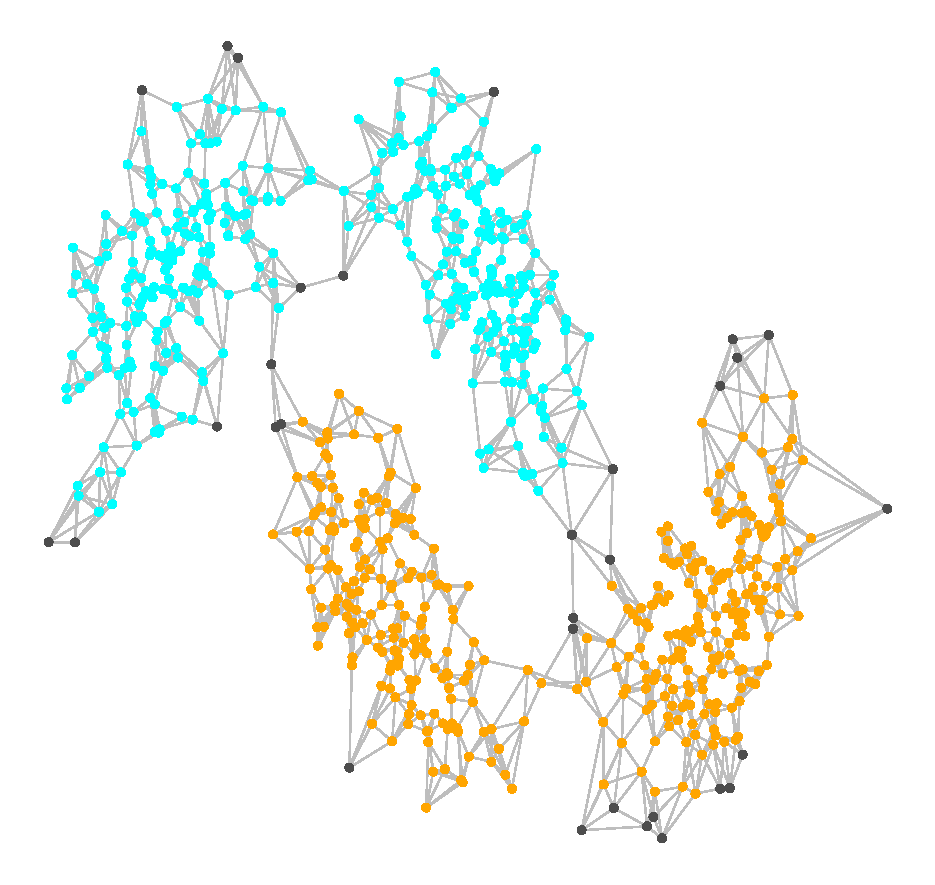
\includegraphics[width=\linewidth,scale = .5]{example3plots/true_density_cluster}
			\caption{}
		\end{subfigure}
		\begin{subfigure}{.24\linewidth}
			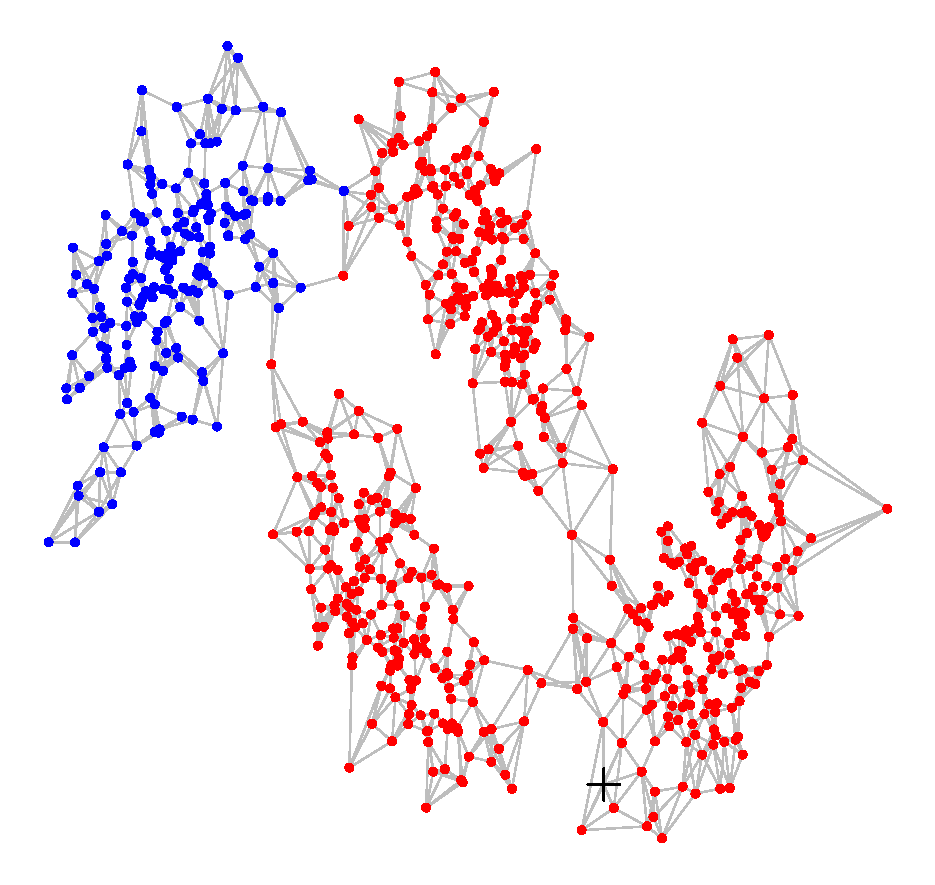
\includegraphics[width=\linewidth,scale = .5]{example3plots/ppr_cluster}
			\caption{}
		\end{subfigure}
		\begin{subfigure}{.24\linewidth}
			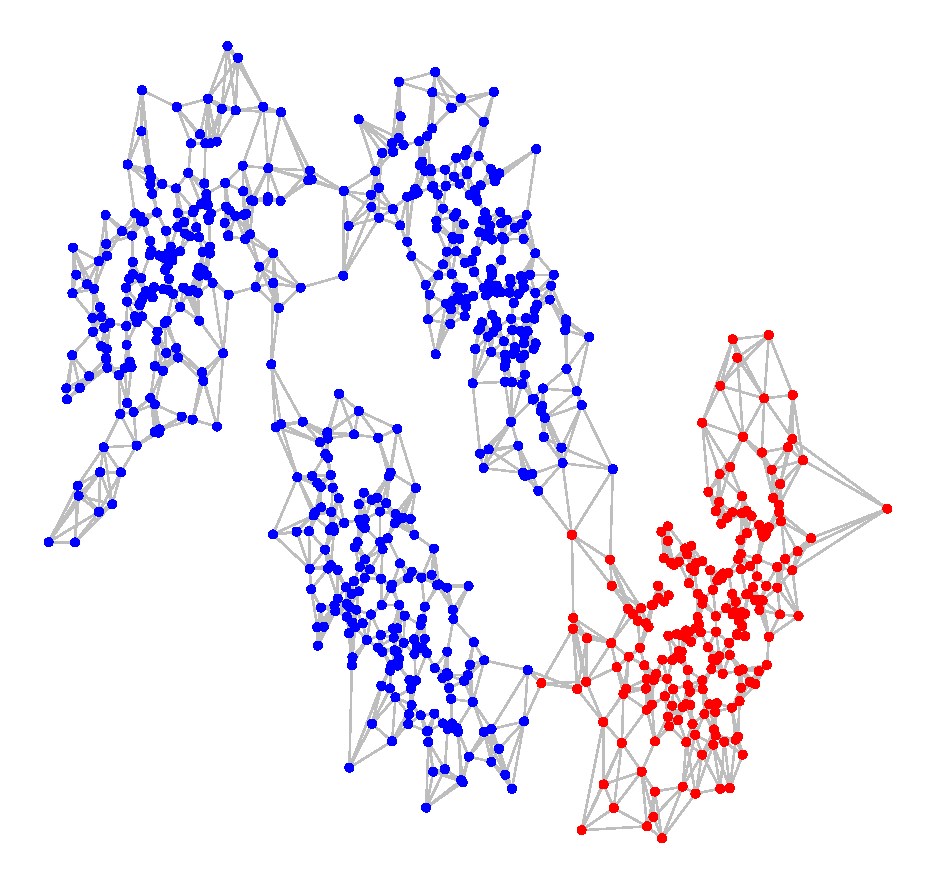
\includegraphics[width=\linewidth,scale = .5]{example3plots/conductance_cluster}
			\caption{}
		\end{subfigure}
		\begin{subfigure}{.24\linewidth}
			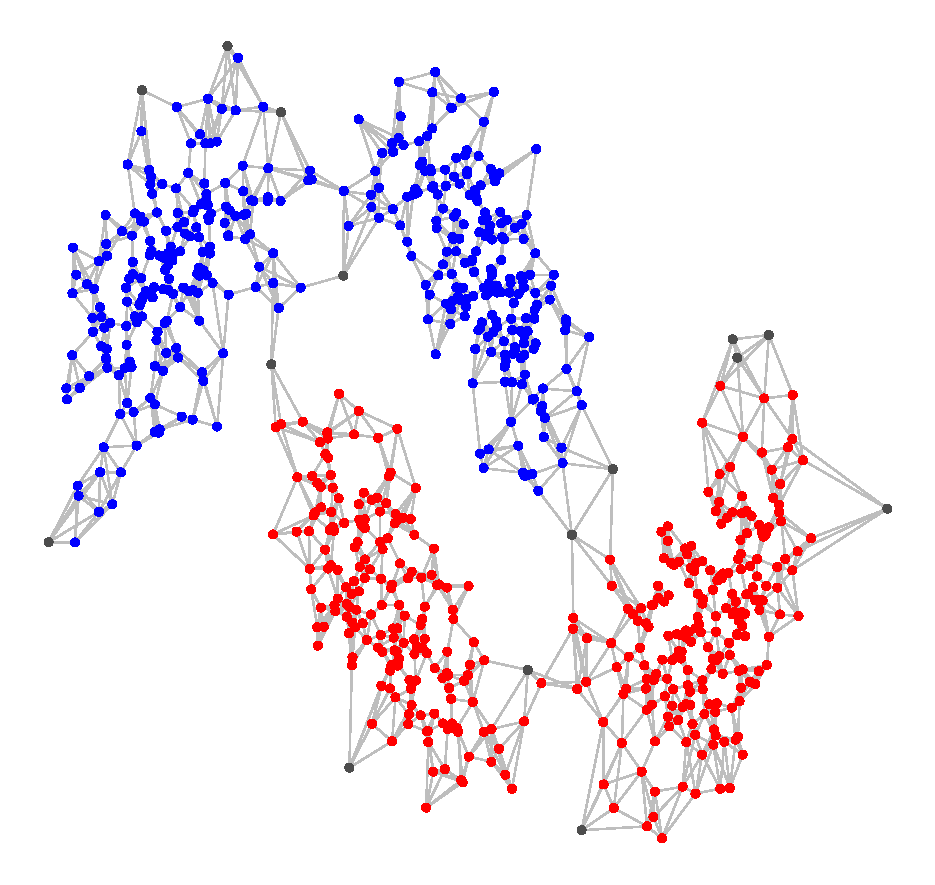
\includegraphics[width=\linewidth,scale = .5]{example3plots/density_cluster}
			\caption{}
		\end{subfigure}
	\caption{}
	\end{adjustbox}
\end{figure}


\section{\textcolor{red}{OLD STUFF}}

\subsection{Volume estimates}
We will fix $\Aset \subset \Rd$ to be an arbitrary set. To simplify expressions, for the $\sigma$-expansion $\Asig$, we will write the set difference between $\Asig$ and the $(\sigma + r)$-expansion $\Aset_{\sigma + r}$ as 
\begin{equation*}
\Asigr := \set{x: 0 < \dist(x, \Asig) \leq r},
\end{equation*}
where as a reminder $\dist(x, \Aset) = \min_{x' \in \Aset} \norm{x - x'}$.

\paragraph{Lemma \ref{lem: interior_of_expansion_sets}.}

We will repeatedly employ Lemma \ref{lem: expansion_sets} and Lemma \ref{lem: Taylor_series} in tandem. As a first example, in Lemma \ref{lem: interior_of_expansion_sets}, we bound the ratio of $\nu(\Aset)$ to $\nu(\Aset_{-\delta})$, where we write $\partial \Aset$ for the boundary of $\Aset$, and for $\delta > 0$ we let
\begin{equation*}
\Aset_{-\delta} : = \set{x \in \Aset: \dist(x, \partial \Aset) > \delta}.
\end{equation*}

This will be useful when we bound $\vol(\Csig)$.

\begin{lemma}
	\label{lem: interior_of_expansion_sets}
	For $\sigma$, $\Asig$ as in Lemma \ref{lem: expansion_sets}, let $r > 0$ satisfy $r \leq \sigma/4d$. Then,
	\begin{equation*}
	\frac{\nu(\Asig)}{\nu(\Aset_{\sigma - r})} \leq 2.
	\end{equation*}
\end{lemma}
\begin{proof}
	Fix $q = \sigma - r$. Then,
	\begin{align*}
	\nu(\Asig) & = \nu(\Aset_{q + \sigma - q}) = \nu(\Aset_q + (\sigma - q)B ) \\
	& \leq \nu(\Aset_q + \frac{(\sigma - q)}{q} \Aset_q) = \left(1 + \frac{\sigma - q}{q}\right)^d \nu(\Aset_q)
	\end{align*}
	where the inequality follows from Lemma \ref{lem: expansion_sets}. Of course, $\sigma - q = r$, and $\frac{r}{q} \leq \frac{1}{2d}$ for $r \leq \frac{1}{4d}$. The claim then follows from Lemma \ref{lem: Taylor_series}.
\end{proof}

\subsection{Proof of Lemma \ref{lem: setup}}

\begin{proof}
	We will write $\Wbf_n = \Dbf_n \Abf_n^{-1}$ for the transition probability matrix over $G_{n,r}$, and let $\widetilde{\Dbf}_n$ and $\widetilde{\Wbf}_n$ be the degree and random walk matrices for the subgraph $\widetilde{G}_{n,r}$.
	
	We introduce \emph{leakage} and \emph{soakage} vectors, defined by
	\begin{align*}
	\ell_t & := e_v (\Wbf_n \widetilde{\mathbf{I}}_n )^t (\mathbf{I}_n - \Dbf_n^{-1} \wDbf_{n}),~ \ell := \sum_{t = 0}^{\infty} (1 - \alpha)^t \ell_t, \\
	s_t & := e_v (\Wbf_n \widetilde{\mathbf{I}}_n )^t (\Wbf_n \widetilde{\mathbf{I}}_n^c),~ s := \sum_{t = 0}^{\infty} (1 - \alpha)^{t} s_t.
	\end{align*}
	where $\mathbf{I}_n$ is the $n \times n$ identity matrix, $\widetilde{\mathbf{I}}_n$ is an $n \times n$ diagonal matrix with $(\widetilde{\mathbf{I}}_n)_{uu} = 1$ if $u \in \Csig[\Xbf]$ and $0$ otherwise, and $\widetilde{\mathbf{I}}_n^c = \mathbf{I}_n - \widetilde{\mathbf{I}}_n$. 
	
	Roughly, the proof of Lemma \ref{lem: setup} will unfold in four steps. The first two will result in the lower bound of (\ref{eqn: lower_bound_PPR_in_cluster}), while the latter two will imply the upper bound in (\ref{eqn: upper_bound_PPR_in_other_cluster}). We briefly summarize the approach before diving into the formal proof:
	
	\begin{enumerate}
		\item For $u \in \Cset[\Xbf]$, we use the results of \cite{zhu2013} to produce the lower bound 
		\begin{equation*}
		\pbf(u) \geq \frac{4}{5}\widetilde{\pi}_{n,r}(u) - \widetilde{\pbf}_{\ell}(u)
		\end{equation*}
		where 
		\begin{equation*}
		\widetilde{\pbf}_{\ell} = \alpha \ell + (1 - \alpha) \widetilde{\pbf}_{\ell} \widetilde{\Wbf}_n
		\end{equation*}
		is the \pprspace random walk over $\widetilde{G}_{n,r}$, and $\ell$ has bounded norm $||\ell||_1 \leq 2\frac{\Phi_{n,r}(\Csig[\Xbf])}{\alpha}$.
		
		\item Since $r < \sigma$, for any $u \in \Cset[\Xbf]$ there are no edges between $u$ and $\Xbf \setminus \Csig[\Xbf]$. Therefore, the page-rank vector $\widetilde{\pbf}_{\ell}$ will not assign more than $||\ell||_1 / d_{\min}(\Csig[\Xbf])$ probability mass to any vertex in $\Cset'[\Xbf]$. This observation will conclude our proof of (\ref{eqn: lower_bound_PPR_in_cluster}).
		\item For vertices $u' \in G_{n,r} / \Csig[\Xbf]$, we can upper bound $p_v(u) \leq p_s(u')$. In particular, this hold for all $u' \in \Cset'[\Xbf]$.
		\item Since $r < \sigma$, there are no edges between $u'$ and $G / \Cset'[\Xbf]$. Therefore, the page-rank vector $p_{s}$ will assign no more than $||s||_1 / d_{\min}(\Csig[\Xbf])$ probability mass to any vertex in $\Cset'[\Xbf]$. Additionally, $s$ has bounded norm $||s||_1 \leq ||\ell||_1$. This will conclude our proof of (\ref{eqn: upper_bound_PPR_in_other_cluster}), and hence Lemma \ref{lem: setup}.
	\end{enumerate}
	
	\paragraph{Step 1}
	We will begin by restating some results of \cite{zhu2013}.
	
	For seed node $v$, we write
	\begin{align} \label{eqn: page_rank_body}
	\widetilde{\pbf}_v & = \alpha e_v + (1 - \alpha) \widetilde{\pbf}_v \widetilde{\Wbf}_n \\
	& = \alpha \sum_{t = 0}^{\infty} (1 - \alpha)^t \left(e_v \widetilde{\Wbf}_n^t \right)
	\end{align}
	
	From Lemma 3.1 of \cite{zhu2013} we have that there exists a good set $\Csig[\Xbf]^g \subseteq \Csig[\Xbf]$ with $\vol(\Csig[\Xbf]^g) \geq \vol(\Csig[\Xbf])/2$ for all $v \in \Csig[\Xbf]^g$, $u \in \Csig[\Xbf]$
	
	\begin{align} \label{eqn: zhu_body}
	p_u & \geq \widetilde{\pbf}_v(u) - \widetilde{\pbf}_{\ell}(u) \nonumber \\
	||\ell||_1 & \leq \frac{2 \widetilde{\Phi}_{n,r}}{\alpha}
	\end{align}
	where $\widetilde{\pbf}_v = (\widetilde{\pbf}_v(u))$ and likewise for $\widetilde{\pbf}_{\ell} = (\widetilde{\pbf}_{\ell}(u))$. (This will be the only time we need to restrict ourselves to this 'good set'.)
	
	Moreover if, as we have specified, $\alpha \leq \widetilde{\Psi}_{n,r}/9$, Lemma 3.2 of \cite{zhu2013} yields a lower bound on $\widetilde{p}$
	\begin{equation} \label{eqn: page_rank_mixes}
	\widetilde{\pbf}_v(u) \geq \frac{4}{5} \widetilde{\pi}_{n,r}(u).
	\end{equation}
	
	\paragraph{Step 2}
	
	We turn to upper bounding $\widetilde{\pbf}_{\ell}(u)$. For any $u \in \Cset[\Xbf]$, we have
	
	\begin{align} \label{eqn: leakage_page_rank_body}
	\widetilde{\pbf}_{\ell}(u) & = \alpha \sum_{t = 0}^{\infty} (1 - \alpha)^t \left(\ell \widetilde{\Wbf}_n^t \right)(u)  \nonumber \\
	& = \|\ell\|_1 \alpha \sum_{t = 0}^{\infty} (1 - \alpha)^t \left(\frac{\ell}{\|\ell\|_1}  \widetilde{\Wbf}_n^t \right)(u)\nonumber \\
	& \overset{\text{(i)}}{=} \|\ell\|_1 \alpha \sum_{t = 1}^{\infty} (1 - \alpha)^t \left(\frac{\ell}{\|\ell\|_1}  \widetilde{\Wbf}_n^t \right)(u)\nonumber \\
	& \overset{\text{(ii)}}{\leq} \|\ell\|_1 \frac{1}{\widetilde{D}_{\min}} 
	\end{align}
	
	where we use $\left(\ell \widetilde{\Wbf}_n^t \right)(u)$ to denote $\ell \widetilde{\Wbf}_n^te_u$.
	
	$\text{(i)}$ follows from the fact that since $r < \sigma$, $\cut(\Cset[\Xbf], G_{n,r} / \Csig[\Xbf]; G_{n,r}) = 0$. Therefore $(\Dbf_n^{-1})_{uu} (\widetilde{\Dbf}_n)_{uu} = 1$, and as a result
	\begin{equation*}
	(\ell \widetilde{\Wbf}_n^0)(u) = \ell(u) = 0.
	\end{equation*}
	To see $\text{(ii)}$, let $q = \frac{\ell}{\|\ell\|_1}  \widetilde{\Wbf}_n^{t-1}$. Then 
	
	\begin{align*}
	\left(\frac{\ell}{\|\ell\|_1}  \widetilde{\Wbf}_n^t \right)(u) & = \left(q \widetilde{\Wbf}_n \right)(u) \\
	& \leq \|q\|_1 \|\widetilde{\Wbf}_{\cdot u}\|_{\infty} \\
	& \overset{\text{(iii)}}{\leq} \frac{1}{\widetilde{D}_{\min}}.
	\end{align*}
	where $\widetilde{\Wbf}_{\cdot u}$ is the $u$th column of $\widetilde{\Wbf}_n$. $\text{(iii)}$ then follows from the fact that any vertex in $\Cset[\Xbf]$ is connected only to vertices in $\Csig[\Xbf]$, and therefore every entry of $\widetilde{\Wbf}_{\cdot u}$ is either $0$ or at most $1 / \widetilde{D}_{\min}$.
	
	
	Combined, (\ref{eqn: leakage_page_rank_body}), (\ref{eqn: page_rank_mixes}), and \eqref{eqn: zhu_body} imply
	\begin{equation*}
	p_v(u) \geq \frac{4}{5} \widetilde{\pi}_{n,r}(u) - 18\frac{ \Phi_{n,r}(\Csig[\Xbf])}{\widetilde{D}_{\min} \alpha}.
	\end{equation*}
	for any $v \in \Csig[\Xbf]$. 
	
	\paragraph{Step 3}
	To get the corresponding upper bound on $p_v(u')$, we will use the soakage vectors $s$ and $s_t$. We will first argue that $s$ is a worse starting distribution -- meaning it puts uniformly more mass outside the cluster -- than simply starting at $v$.
	
	\begin{lemma} \label{lem: gained mass is soaked_body}
		For all $u' \notin \Csig[\Xbf]$,
		\begin{equation}
		\pbf_v(u') \leq \pbf_{s}(u').
		\end{equation}
	\end{lemma}
	
	\begin{proof}
		
		We have
		\begin{align*}
		\pbf_v(u') & = \alpha \sum_{T=0}^{\infty} (1 - \alpha)^T (e_v \Wbf_n^T)(u)\\
		& \overset{(i)}{=} \alpha \sum_{T=1}^{\infty} (1 - \alpha)^T (e_v \Wbf_n^T)(u')
		\end{align*}
		
		where $(i)$ follows from $v \in \Csig$ , $u \not\in \Csig$ and therefore $e_v(u) = 0$. 
		
		Lemma \ref{lem: sum_of_soakages} allows us to make the transition to sums of soakage vectors. 
		\begin{lemma}
			
			Let $G = (V,E)$ be a graph, with associated random walk matrix $W$.
			
			For any $T \geq 1$, $q$ vector, $S \subset V$, and $s_t = s_t(S^c,q)$
			\begin{equation}
			qW^T = \sum_{t = 0}^{T - 1} s_t W^{T - t - 1} + q(W I_S)^T
			\end{equation}
		\end{lemma}
		We prove Lemma \ref{lem: sum_of_soakages} after completing the proof of Lemma \ref{lem: gained mass is soaked_body}.
		
		Now, along with the fact $u \not\in \Csig$, we have
		
		\begin{equation*}
		\left(e_v \Wbf_n^T \right)(u') = \sum_{t = 0}^{T - 1} \left(s_t \Wbf_n^{T - t - 1} \right)(u')
		\end{equation*}
		
		and so
		
		\begin{align*}
		\pbf_v(u) & = \alpha \sum_{T=1}^{\infty} (1 - \alpha)^T \left( \sum_{t = 0}^{T - 1} s_t \Wbf^{T - t - 1} \right)(u') \\
		& = \alpha \sum_{t=0}^{\infty} \sum_{T = t + 1}^{\infty} (1 - \alpha)^T \left( s_t \Wbf^{T - t - 1} \right)(u')\\
		& = \alpha \sum_{t=0}^{\infty} \sum_{\Delta = 0}^{\infty} (1 - \alpha)^{\Delta + t + 1} \left( s_t \Wbf_n^{\Delta} \right)(u') \\
		& \leq \alpha \sum_{t=0}^{\infty} \sum_{\Delta = 0}^{\infty} (1 - \alpha)^{\Delta + t } \left( s_t \Wbf_n^{\Delta} \right)(u') \\
		& = \alpha \sum_{\Delta = 0}^{\infty} (1 - \alpha)^{\Delta} \left(s \Wbf_n^{\Delta}\right)(u') \\
		& = \pbf_s(u')
		\end{align*}
	\end{proof}
	
	\begin{proof}[Proof of Lemma \ref{lem: sum_of_soakages}]
		Proceed by induction. When $T = 1$,
		
		\begin{align*}
		qW & = q(WI_S) + q(WI_{S^c}) \\
		& = q(W I_S)^T + s_0 
		\end{align*}
		
		Assume true for $T_0$. For $T = T_0 + 1$,
		
		\begin{align*}
		qW^T & = qW^{T_0}W \\
		& = \left\{ \sum_{t = 0}^{T_0 - 1} s_t W^{T_0 - 1 - t} + q(WI_S)^{T_0} \right\} W \\
		& =  \sum_{t = 0}^{T_0 - 1} s_t W^{T - 1 - t} + q(WI_S)^{T_0}(WI_S + WI_{S^c}) \\
		& =  \sum_{t = 0}^{T - 1} s_t W^{T - 1 - t} + q(WI_S)^{T}
		\end{align*}
	\end{proof}
	
	\paragraph{Step 4}
	
	Just as we upper bounded the probability mass $\widetilde{\pbf}_{\ell}$ could assign to any one vertex, we can upper bound 
	
	\begin{align} \label{eqn: soakage_page_rank_body}
	\pbf_{s}(u') & = \alpha \sum_{t = 0}^{\infty} (1 - \alpha)^t \left(s \Wbf_n^t \right)(u') \nonumber \\
	& = \|s\|_1 \alpha \sum_{t = 0}^{\infty} (1 - \alpha)^t \left(\frac{s}{\|s\|_1} {\Wbf}_n^t \right)(u')\nonumber \\
	& = \|s\|_1 \alpha \sum_{t = 1}^{\infty} (1 - \alpha)^t \left(\frac{s}{\|s\|_1}  {\Wbf}_n^t \right)(u')\nonumber \\
	& \leq \|s\|_1 \frac{1}{\widetilde{D}_{\min}}.
	\end{align}
	
	Finally, letting $q_t = e_v (\Wbf_n \widetilde{\mathbf{I}}_n)^t$ for ease of notation, we have
	\begin{align*}
	\|s_t\|_1 & = \|q_t (\Wbf_n \widetilde{\mathbf{I}}_n)\|_1 \\
	& = \sum_{u' \in \Xbf} \sum_{u \in \Xbf} q_t(u) (\Wbf_n \widetilde{\mathbf{I}}_n)(u, u')\\
	& = \sum_{u' \in \Xbf / \Csig[\Xbf]} \sum_{u \in \Csig[\Xbf]} \frac{q_t(u)}{(\Dbf_n)_{uu}} \1(e_{u,u'} \in G_{n,r}) \\
	& = \sum_{u \in \Csig[\Xbf]} \frac{q(u) \left((\Dbf_n)_{uu} - (\widetilde{\Dbf}_n)_{uu} \right)}{(\Dbf_n)_{uu}} \\
	& = \|q_t (I - \Dbf_n^{-1} \widetilde{\Dbf}_n)\|_1 = \|\ell_t\|_1.
	\end{align*}
	
	and as a result $\|s\|_1 = \|\ell\|_1$. Combining with $\|\ell\|_1 \leq 2 \frac{\widetilde{\Phi}_{n,r}}{\alpha}$ and (\ref{eqn: soakage_page_rank_body}) yields the desired upper bound.
\end{proof}

\paragraph{Proof of Theorem \ref{thm: consistent_recovery_of_density_clusters}.}

We note that by Theorems \ref{thm: conductance_upper_bound} and \ref{thm: inverse_mixing_time_lower_bound_nonconvex}, 
\begin{equation*}
\kappa_2(\Cset) \geq \frac{\Phi_{n,r}(\Csig[\Xbf])}{\Psi_{n,r}(\Csig[\Xbf])}.
\end{equation*}
As a result Lemma \ref{lem: setup} implies
\begin{align}
\label{eqn: theorem_4_1}
p_u & \geq \frac{4}{5} \widetilde{\pi}_{n,r}(u) - \frac{18 \kappa_2(\Cset)}{\widetilde{D}_{\min}} ~~~~~~ (u \in \Cset[\Xbf]) \nonumber \\
p_{u'} & \leq \frac{18 \kappa_2(\Cset)}{\widetilde{D}_{\min}} ~~~~~~~~~~~~~~~~~~~~~ (u' \in \Cset'[\Xbf])
\end{align}

We turn to bounding $\widetilde{\pi}_{n,r}(u)$. Clearly,
\begin{align*}
\widetilde{\pi}_{n,r}(u) & \geq \frac{\widetilde{D}_{\min}}{\widetilde{\vol}_{n,r}(\Csig[\Xbf])} \\
& \geq \frac{\widetilde{D}_{\min}}{\wn \widetilde{D}_{\max}}.
\end{align*}
Application of Lemma \ref{lem: ball_bounds_in_probability} then yields
\begin{equation}
\label{eqn: theorem_4_2}
\widetilde{\pi}_{n,r}(u) \geq 8 \frac{\lambda_{\sigma}}{\nu(\Csig) \Lambda_{\sigma}^2}
\end{equation}
as well as
\begin{equation}
\label{eqn: theorem_4_3}
\frac{1}{\widetilde{D}_{\min}} \leq \frac{2}{\nu_d r^d \lambda_{\sigma}}
\end{equation}
with probability tending to $1$ as $n \to \infty$, for all $u \in \Cset[\Xbf]$ (indeed, all $u \in \Csig[\Xbf]$.)

Combining \eqref{eqn: theorem_4_1}, \eqref{eqn: theorem_4_2} and \eqref{eqn: theorem_4_3}, along with the requirement on $\kappa_2(\Cset)$ given by \eqref{eqn: kappa2_ub}, we have
\begin{align*}
p_u & \geq 3/5 \frac{\lambda_{\sigma}}{\nu(\Csig) \Lambda_{\sigma}^2} \\
p_{u'} & \leq 1/5 \frac{\lambda_{\sigma}}{\nu(\Csig) \Lambda_{\sigma}^2}
\end{align*}
for any $u \in \Cset$, $u' \in \Cset'$. As a result, if $\pi_0 \in (2/5, 3/5)\cdot \frac{\lambda_{\sigma}}{\nu(\Csig) \Lambda_{\sigma}^2}$, as $n \to \infty$ with probability tending to one any sweep cut of the form of \eqref{eqn: sweep_cuts}, including the output set $\widehat{C}$, will successfully recover $\Cset$ in the sense of \eqref{eqn: consistent_density_cluster_recovery}.

\clearpage
\bibliographystyle{plain}
\bibliography{../local_spectral_bibliography}

\end{document}